                \documentclass[t]{beamer}
%
% Choose how your presentation looks.
%
% For more themes, color themes and font themes, see:
% http://deic.uab.es/~iblanes/beamer_gallery/index_by_theme.html
%
\mode<presentation>
{
  \usetheme{Boadilla}      % or try Darmstadt, Madrid, Warsaw, ...
  \usecolortheme{default} % or try albatross, beaver, crane, ...
  \usefonttheme{default}  % or try serif, structurebold, ...
  \setbeamertemplate{navigation symbols}{}
  \setbeamertemplate{caption}[numbered]
  \setbeamerfont{bibliography item}{size=\footnotesize}
  \setbeamerfont{bibliography entry author}{size=\footnotesize}
  \setbeamerfont{bibliography entry title}{size=\footnotesize}
  \setbeamerfont{bibliography entry location}{size=\footnotesize}
  \setbeamerfont{bibliography entry note}{size=\footnotesize}
} 

\setbeamertemplate{footnote}{%
  \tiny%
  \parindent 1em\noindent%
  \raggedright
  \hbox to 1.8em{\hfil\insertfootnotemark}\insertfootnotetext\par%
}%
\setlength\footnotesep{0pt}

\usefonttheme[onlymath]{serif}

\usepackage[english]{babel}
\usepackage[utf8x]{inputenc}
\usepackage{caption}
\usepackage{booktabs}
\usepackage{biblatex}
%\usepackage{natbib}
\usepackage{multirow}
\usepackage{ifthen}
\usepackage{bibentry}
\usepackage{array}
%\bibliographystyle{achemso}
\usepackage{chngcntr}

%%%%%%%%%%%%%%%%%%%%%%%%%%%%%%%
%% Center Titles for Frames%%%
%%%%%%%%%%%%%% %%%%%%%%%%%%%%%%%
\makeatletter 
\long\def\beamer@@frametitle[#1]#2{% 
  \beamer@ifempty{#2}{}{% 
    \gdef\insertframetitle{\centering{#2\ifnum\beamer@autobreakcount>0\relax{}\space\usebeamertemplate*{frametitle continuation}\fi}}% 
  \gdef\beamer@frametitle{#2}% 
  \gdef\beamer@shortframetitle{#1}% 
}% 
}

\newcommand\blfootnote[1]{%
  \begingroup
  \renewcommand\thefootnote{}\footnote{#1}%
  \addtocounter{footnote}{-1}%
  \endgroup
}
 
\makeatother 
%%%%%%%%%%%%%%%%%%%%%%%%%%%%%%%%%%%%%%%%%%%%%
%\usepackage[backend=bibtex,style=science]{biblatex}
%\bibliography{research}
\captionsetup{font=scriptsize,labelfont=scriptsize}

\title[Simulating XAS in OCDFT]{Development and Applications of Orthogonality Constrained Density Functional Theory for the Accurate Simulation X-Ray Absorption Spectroscopy}
\author{Wallace Derricotte}
\institute{Dissertation Defense}
\date{June 28th, 2017}

\newcommand{\bra}[2][0]
{\ifthenelse{\equal{#1}{0}}{\left\langle #2 \right|}
{\ifthenelse{\equal{#1}{1}}{\big\langle #2 \big|}
{\ifthenelse{\equal{#1}{2}}{\Big\langle #2 \Big|}
{\ifthenelse{\equal{#1}{3}}{\bigg\langle #2 \bigg|}
{\ifthenelse{\equal{#1}{4}}{\Bigg\langle #2 \Bigg|}
{Error}}}}}
}

% <#2|#3|#4>, #1 gives the size of the bracket
\newcommand{\bracket}[4][0]
{\ifthenelse{\equal{#1}{0}}{\left\langle #2 \middle| #3 \middle| #4 \right\rangle}
{\ifthenelse{\equal{#1}{1}}{\big\langle #2 \big| #3 \big| #4 \big\rangle}
{\ifthenelse{\equal{#1}{2}}{\Big\langle #2 \Big| #3 \Big| #4 \Big\rangle}
{\ifthenelse{\equal{#1}{3}}{\bigg\langle #2 \bigg| #3 \bigg| #4 \bigg\rangle}
{\ifthenelse{\equal{#1}{4}}{\Bigg\langle #2 \Bigg| #3 \Bigg| #4 \Bigg\rangle}
{Error}}}}}
}

% <#2|#3>, #1 gives the size of the bracket
\newcommand{\braket}[3][0]
{\ifthenelse{\equal{#1}{0}}{\left\langle #2 \middle| #3 \right\rangle}
{\ifthenelse{\equal{#1}{1}}{\big\langle #2 \big| #3 \big\rangle}
{\ifthenelse{\equal{#1}{2}}{\Big\langle #2 \Big| #3 \Big\rangle}
{\ifthenelse{\equal{#1}{3}}{\bigg\langle #2 \bigg| #3 \bigg\rangle}
{\ifthenelse{\equal{#1}{4}}{\Bigg\langle #2 \Bigg| #3 \Bigg\rangle}
{Error}}}}}
}

% |#2>, #1 gives the size of the bracket
\newcommand{\ket}[2][0]
{\ifthenelse{\equal{#1}{0}}{\left| #2 \right\rangle}
{\ifthenelse{\equal{#1}{1}}{\big| #2 \big\rangle}
{\ifthenelse{\equal{#1}{2}}{\Big| #2 \Big\rangle}
{\ifthenelse{\equal{#1}{3}}{\bigg| #2 \bigg\rangle}
{\ifthenelse{\equal{#1}{4}}{\Bigg| #2 \Bigg\rangle}
{Error}}}}}
}

\graphicspath{{figures/}}
\counterwithin*{footnote}{page}
\newcommand\footcite[1]{\footnote{\bibentry{#1}\label{\thepage:#1}}}
\newcommand\secondcite[1]{\textsuperscript{\ref{\thepage:#1}}}
\begin{document}
%\nobibliography{defense_talk}

\begin{frame}
  \titlepage
\end{frame}

\begin{frame}{X-ray Absorption Mechanism: Core-Excited States}
\begin{figure}
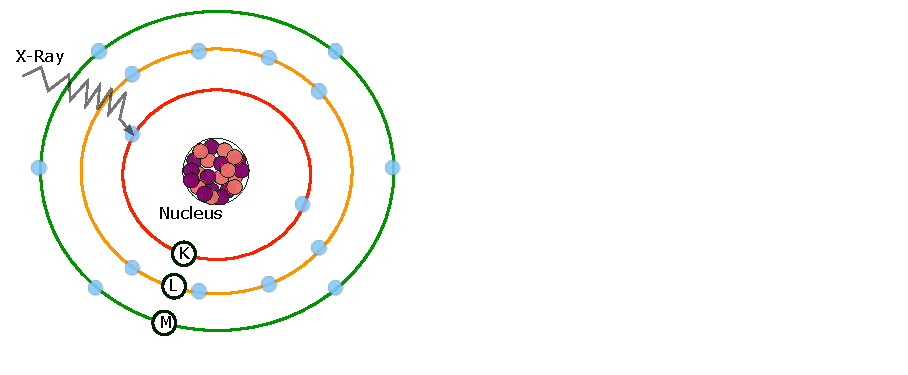
\includegraphics[scale=0.7]{core_mechanism_1.pdf}
\begin{itemize}
\item X-ray photons excite core electrons (i.e. 1s, 2s, 2p)
\item Core orbitals are close to nuclei, experience strong Coulombic attraction
\end{itemize}
\end{figure}
\end{frame}

\begin{frame}{X-ray Absorption Mechanism: Core-Excited States}
\begin{figure}
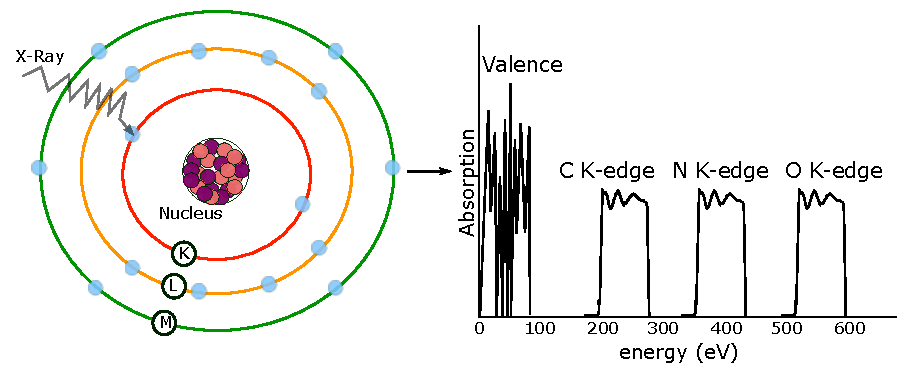
\includegraphics[scale=0.7]{core_mechanism_2.pdf}
\end{figure}
\begin{itemize}
\item X-ray photons excite core electrons (i.e. 1s, 2s, 2p)
\item Core orbitals are close to nuclei, experience strong Coulombic attraction
\item Produces \textbf{element specific} edge jump in absorption spectrum
		\begin{itemize}
		\item X-ray notation based on principal quantum number\footnotemark (K=1, L=2, M=3)
		\end{itemize}
\end{itemize}
\footnotetext{J. Stohr. \textit{NEXAFS Spectroscopy}; Springer: \textbf{1992}}
\end{frame}

\begin{frame}{Fine Structure of the XAS Edge}
\begin{figure}
\includegraphics[scale=0.7]{fine_structure.pdf}
\end{figure}
\begin{itemize}
\item Edge has 3 distinct regions: Pre, Rising, and Extended Edges
\item Near-edge X-ray absorption fine structure (NEXAFS) spectroscopy studies the pre and rising edge regions
\item Extended-edge X-ray absorption fine structure (EXAFS) spectroscopy studies the extended edge region\footnotemark
\end{itemize}
\footnotetext{B. K. Teo. \textit{EXAFS: Basic Principles and Data Analysis}; Springer: \textbf{2012}}
\end{frame}

\begin{frame}{Computational Methods for Simulating NEXAFS}
\begin{itemize}
\item Interpretation of NEXAFS requires knowledge of core-excitation energies, transition dipole moments, and orbital character of transition
\item Wavefunction/Green's Function Methods
		\begin{itemize}
		\item Linear Response Coupled Cluster (LR-CC)
		\item Algebraic Diagrammatic Construction (ADC)
		\item RASSCF
		\item SOS-CIS(D)
		\end{itemize}
\item Density Functional Theory Methods
		\begin{itemize}
		\item Linear Response Time-Dependent DFT (TDDFT)
		\item Real-Time TDDFT
		\end{itemize}
\item Hartree--Fock (HF) Based Approaches
		\begin{itemize}
		\item HF Static Exchange Method (HF-STEX)
		\item Maximum Overlap $\Delta$SCF
		\end{itemize}
\item All theoretical methods face unique theoretical challenges when calculating core excited states
\end{itemize}
\end{frame}

\begin{frame}{Theoretical Challenges: Orbital Relaxation}
\begin{itemize}
\item Orbital relaxation effects can be understood formally as the change in orbital energies when changing the number of electrons
\end{itemize}
\centering
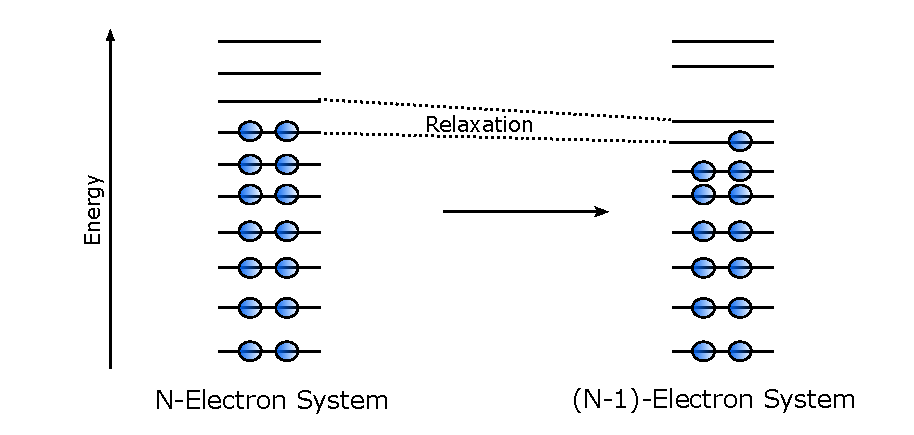
\includegraphics[width=0.8\linewidth]{orbital_relaxation_diagram.pdf}
\begin{itemize}
\item Remaining orbitals are drawn closer to the nucleus which becomes more effectively screened
\end{itemize}
\end{frame}

\begin{frame}{Orbital Relaxation Effects in Core-Excited States}
\begin{figure}[!t]
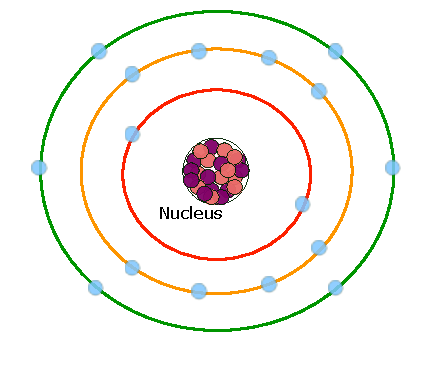
\includegraphics[scale=0.7]{core_hole_generation_1.pdf}
\end{figure}
\begin{itemize}
\item Effective nuclear charge ($Z_{\rm eff}$) on any electron can be approximated as:
\begin{equation}
Z_{\rm eff} = Z - \sigma
\end{equation}
\item where Z is the number of protons and $\sigma$ is the average number of electrons b/w the nucleus and the electron in question
\end{itemize}
\end{frame}

\begin{frame}{Orbital Relaxation Effects in Core-Excited States}
\begin{figure}[!t]
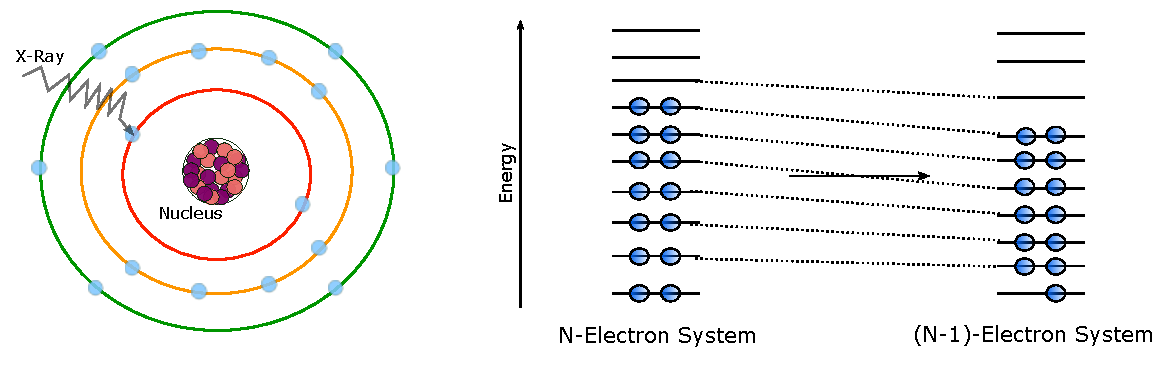
\includegraphics[width=\linewidth]{core_hole_generation_2.pdf}
\end{figure}
\begin{itemize}
\item Generation of a core-hole causes a decrease in the shielding of the nuclei 
\item Causes significant rearrangement in all higher lying orbitals, known as \textbf{orbital relaxation}
\item It was shown that for a N atom, this effect can be on the order of 12-15 eV
\end{itemize}
\end{frame}

\begin{frame}{Theoretical Challenges: Relativistic Effects}
\begin{figure}
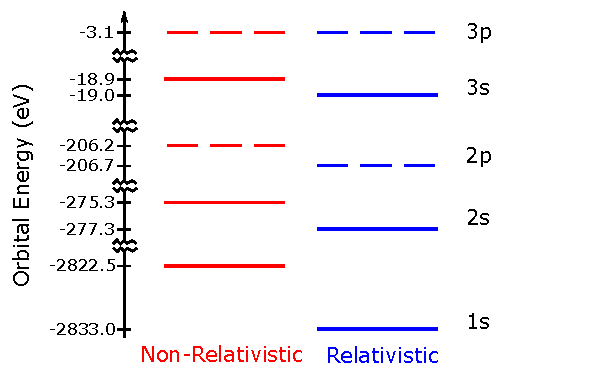
\includegraphics[scale=0.8]{relativistic_contraction.pdf}
\caption*{Orbital energies of Cl$^{-}$ from non-relativistic and scalar relativistic Hartree--Fock calculations.}
\end{figure}
\begin{itemize}
\item Core orbitals experience large \textbf{relativistic} contraction while the valence orbitals remain relatively uneffected
\item Results in increase in core-excitation energy
\end{itemize}
\end{frame}

\begin{frame}{Theoretical Challenges: Relativistic Effects}
\begin{table}
\centering
\caption{Non-relativistic (NR) and relativistic (R) energies (in eV) of the lowest lying core orbital and lowest unoccupied molecular orbital (LUMO) of water (H$_2$O) and silane (SiH$_4$) molecules calculated using spin-unrestricted Hartree--Fock (UHF) with the 3-21G basis set. Scalar relativistic effects are included by use of the 2$^{\rm nd}$ order Douglas-Kroll-Hess Hamiltonian.\footnotemark All calculations were performed using the ORCA software package.}
\begin{tabular}{ccccc}
\toprule
& \multicolumn{2}{c}{H$_2$O} & \multicolumn{2}{c}{SiH$_4$} \\ \cmidrule(lr){2-3} \cmidrule(lr){4-5}
& O 1s & LUMO & Si 1s & LUMO \\
\hline
NR-UHF & $-$555.88 & 7.17 & $-$1858.20 & 5.02\\
R-UHF & $-$556.34 & 7.16 & $-$1863.04 & 5.03\\
\bottomrule
\end{tabular}
\label{tab:rel_effects}
\end{table}
\begin{itemize}
\item Effect is more pronounced in heavier elements
\item Small but non-negligible effect on light elements 
\end{itemize}
\footnotetext{M. Reiher. \textit{Theor. Chem. Acc.}. \textbf{2006}}
\end{frame}

\begin{frame}{Theoretical Challenges: Assigning Excited States}
\begin{itemize}
\item Excited states are often assigned based on MO plots relative to the ground state
\end{itemize}
\centering
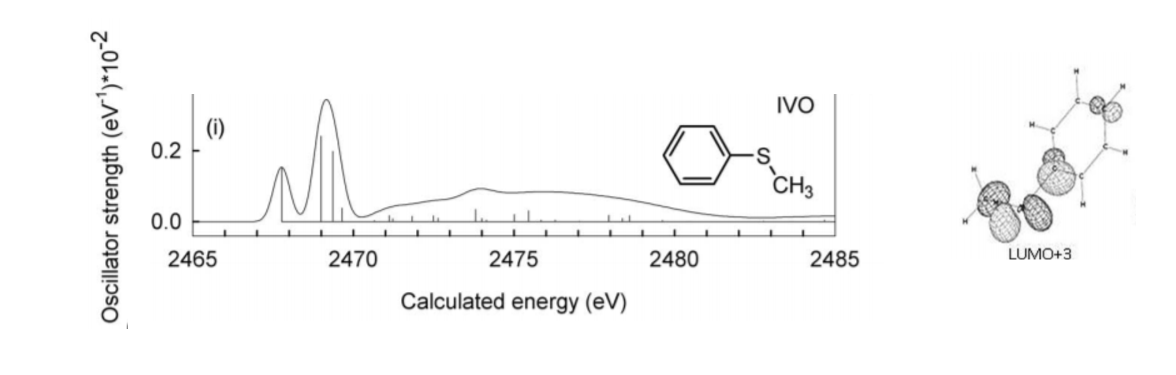
\includegraphics[width=\linewidth]{behyan_fig.pdf}
\begin{itemize}
\item LUMO+3 for methylsulfanyl benzene above was assigned as $\pi^*$(C=C),\footnotemark  but other contributions are clearly present
\item Two issues with this type of assignment
		\begin{itemize}
		\item Assignments based on MO plots are potentially ambiguous
		\item Approach is not systematic/reproducible
		\end{itemize}
\end{itemize}
\footnotetext{S. Behyan; Y. Hu; S. G. Urquhart. \textit{J. Chem. Phys.} \textbf{2013}}
\end{frame}

\begin{frame}{Overview of Dissertation Work}
\centering
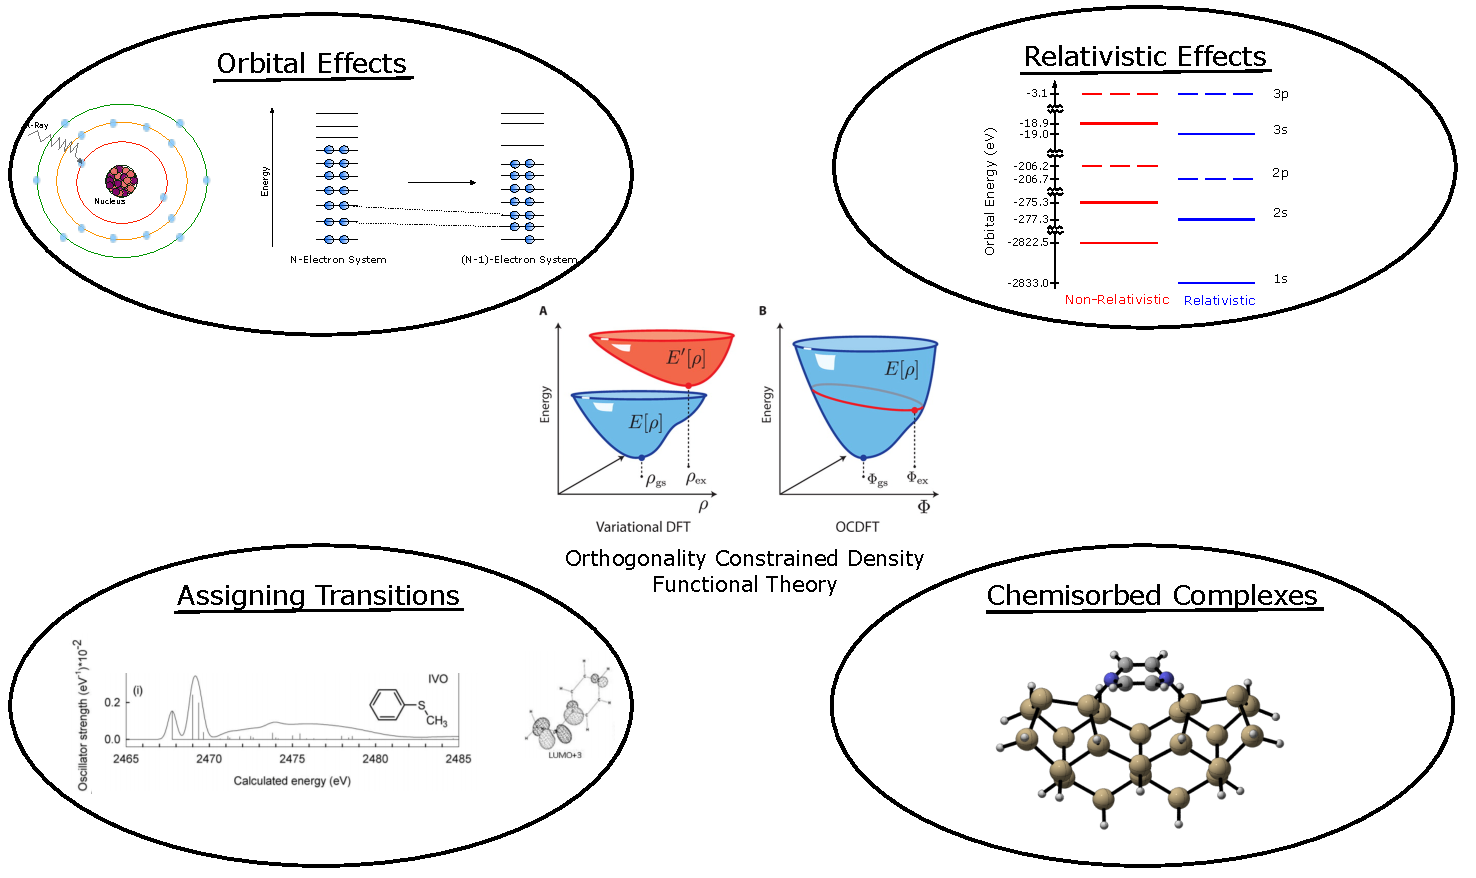
\includegraphics[width=\linewidth]{dissertation_work_overview.pdf}
\end{frame}

\begin{frame}{Orthogonality Constrained Density Functional Theory}
\centering
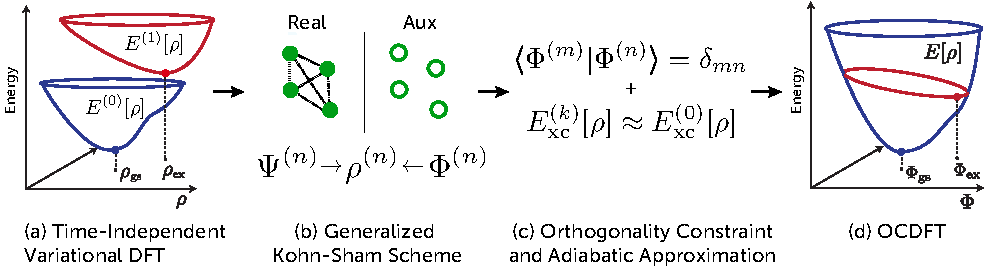
\includegraphics[width=\linewidth]{figure_1.pdf}
\begin{itemize}
\item Variational time-independent (TI) formulation of density functional theory (DFT)\footnotemark
\item This choice of constraint prevents \textbf{variational collapse} of the excited state SCF
\item OCDFT excited state functional can be written as:
\begin{align}
\nonumber
E^{(n)}_{\rm OCDFT}[\{\phi^{(n)}_i\}]=& \sum_{\mu \nu} D^{(n)}_{\mu \nu}(T_{\mu \nu} + V_{\mu \nu}) + E_{\rm coul}[\rho^{(n)}] + E^{(0)}_{\rm xc}[\rho^{(n)}]. 
\end{align}
\end{itemize}
\footnotetext{F. A. Evangelista; P. Shushkov; and J. C. Tully. \textit{J. Phys. Chem. A.} \textbf{2013}}
\end{frame}

\begin{frame}{OCDFT: Minimal Orthogonality Conditions}
\centering
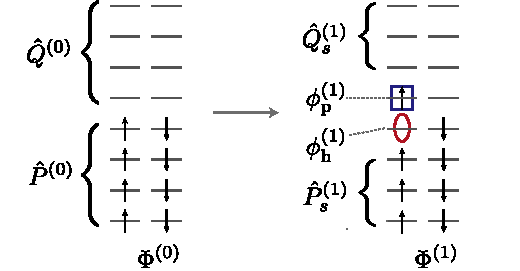
\includegraphics[width=0.6\linewidth]{hole_particle_orthogonality.pdf}
\begin{itemize}
\item Enforcing orthogonality introduces a \textit{hole} ($\phi_{\rm h}^{(1)}$) and \textit{particle} ($\phi_{\rm p}^{(1)}$) orbital that must satisfy the following:
\begin{align}
\label{eq:pq_conditions1}
\hat{Q}^{(0)}\phi_{\rm h}^{(1)} = 0,\\
\label{eq:pq_conditions2}
\hat{P}^{(0)}\phi_{\rm p}^{(1)} = 0,
\end{align}
\item In quasiparticle formalism, $\phi_{\rm h}^{(1)}$ and $\phi_{\rm p}^{(1)}$ define the single excitation
\end{itemize}
\end{frame}

\begin{frame}{OCDFT: Hole and Particle Orbitals in Practice}
\begin{figure}
\centering
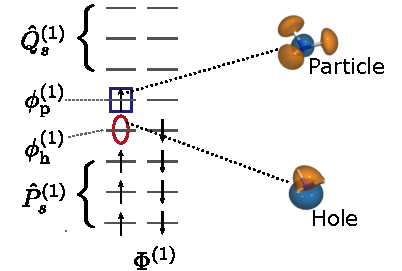
\includegraphics{hole_particle_practice.pdf}
\caption*{Particle orbitals for first excited state in NH$_3$. Calculated using OCDFT at B3LYP/3-21G level of theory} 
\end{figure}
\begin{itemize}
\item Visual representation of each single excited state
\item $\phi_{\rm h}^{(1)}$ and $\phi_{\rm p}^{(1)}$ are variationally optimized for the excited state
\end{itemize}
\end{frame}

\begin{frame}{Treatment of Orbital Relaxation in OCDFT}
\centering
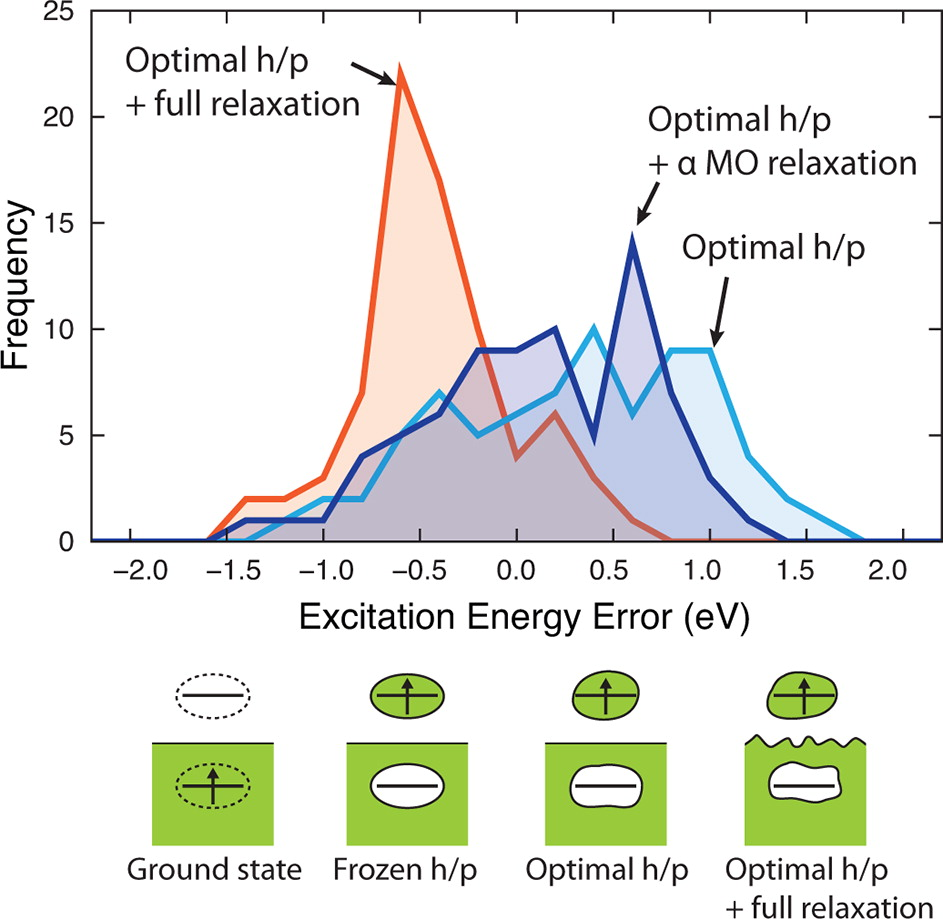
\includegraphics[scale=0.65]{relaxation_original.jpeg}
\begin{itemize}
\item Original tests on valence excitation showed full inclusion of relaxation effects yielded best results\footnotemark
\item If the theory is extended to core excitation we can benefit from full inclusion of orbital relaxation
\end{itemize}
\footnotetext{F. A. Evangelista; P. Shushkov; and J. C. Tully. \textit{J. Phys. Chem. A.} \textbf{2013}}
\end{frame}

\begin{frame}{Developing OCDFT For Core-Excited States}
\centering
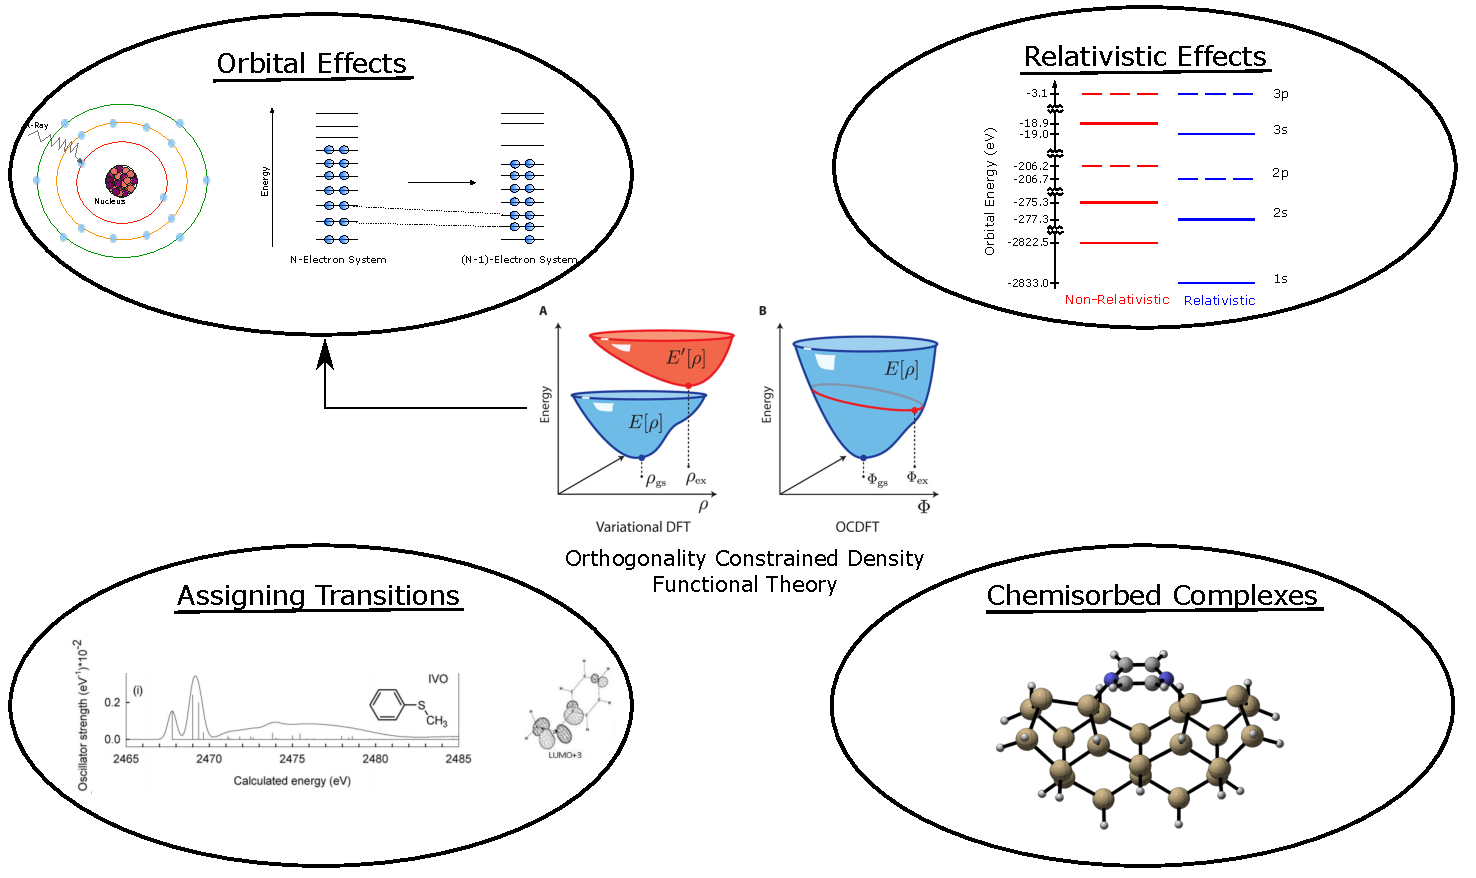
\includegraphics[width=\linewidth]{project_intro_1.pdf}
\end{frame}

\begin{frame}{Extension of OCDFT For NEXAFS Spectral Simulation}
\begin{itemize}
\item Must introduce two new features to OCDFT to calculate NEXAFS spectra
		\begin{itemize}
		\item Previous implementation starts from \textit{highest lying} hole orbital (highest hole eigenvalue) however for core excitations we need to select the \textit{lowest lying} hole orbital (lowest hole eigenvalue)
		\item Algorithm must be generalized to multiple excited states
		\end{itemize}
\end{itemize}
\centering
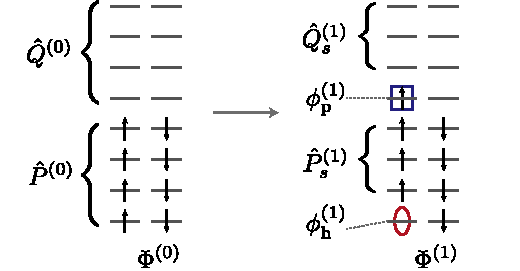
\includegraphics[scale=0.85]{Figure1.pdf}
\blfootnote{W. D. Derricotte and F. A. Evangelista. \textit{Phys. Chem. Chem. Phys.} \textbf{2015}}
\end{frame}

\begin{frame}{Extension of OCDFT For NEXAFS Spectral Simulation}
\begin{figure}[!t]
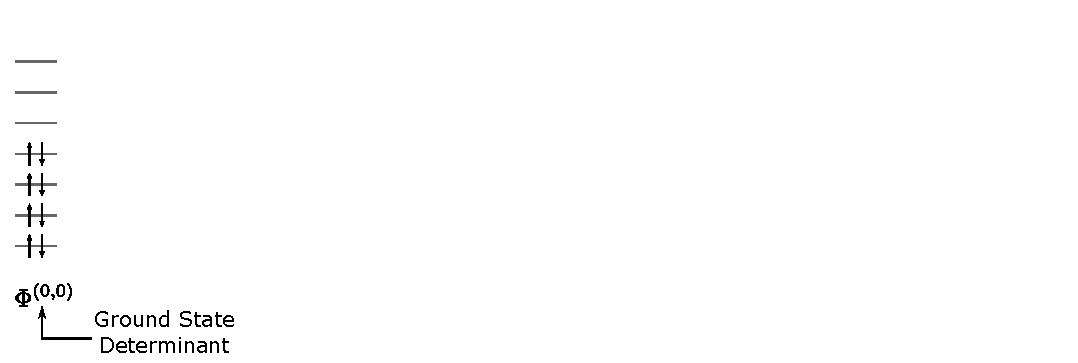
\includegraphics[scale=0.65]{CMHP_alg1.pdf}
\end{figure}
\begin{itemize}
\item First, perform a ground state DFT calculation to obtain the ground state determinant $\Phi^{(0,0)}$
\item Utilizing notation $\Phi^{(i,a)}$ where $i$ and $a$ are hole and particle indices respectively
\end{itemize}
\blfootnote{W. D. Derricotte and F. A. Evangelista. \textit{Phys. Chem. Chem. Phys.} \textbf{2015}}
\end{frame}

\begin{frame}{Extension of OCDFT For NEXAFS Spectral Simulation}
\begin{figure}[!t]
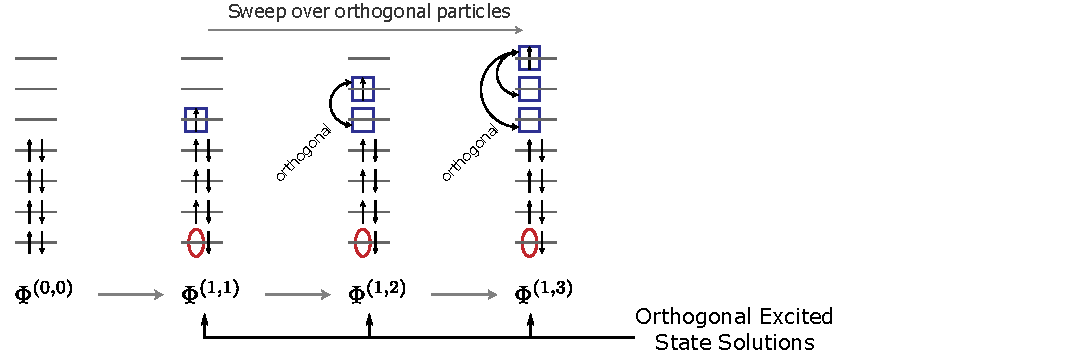
\includegraphics[scale=0.65]{CMHP_alg2.pdf}
\end{figure}
\begin{itemize}
\item Perform a sweep of $n_u$ particle orbitals to produce a series of core-excited solutions: $\Phi^{(1,1)}, \Phi^{(1,2)}, \ldots, \Phi^{(1,n_{\rm u})}.$
\item Characterized by particle orbitals that produce an orthogonal set:
\begin{align}
\braket[1]{\phi^{(1,a)}_{\rm p}}{\phi^{(1,b)}_{\rm p}} &= \delta_{ab}, &\forall a,b \leq n_{\rm u}.
\end{align}
\end{itemize}
\blfootnote{W. D. Derricotte and F. A. Evangelista. \textit{Phys. Chem. Chem. Phys.} \textbf{2015}}
\end{frame}
\begin{frame}{Extension of OCDFT For NEXAFS Spectral Simulation}
\begin{figure}[!t]
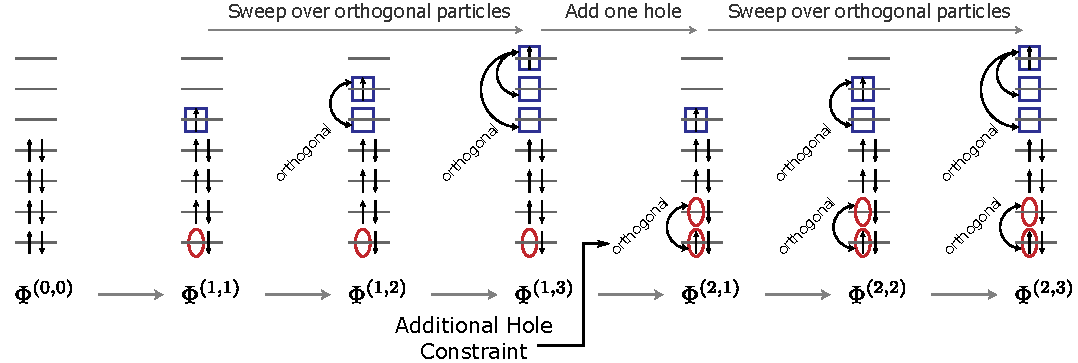
\includegraphics[scale=0.65]{CMHP_alg3.pdf}
\end{figure}
\begin{itemize}
\item Increase core index by one and sweep through another series of core-excited solutions: $\Phi^{(2,1)}, \Phi^{(2,2)}, \ldots, \Phi^{(2,n_{\rm u})}.$
\item Where an additional constraint is added to the hole orbital to be orthogonal to the hole orbital of the first sweep:
\begin{align}
\braket[1]{\phi^{(1,1)}_{\rm h}}{\phi^{(2,a)}_{\rm h}} &=0,&\forall a \leq n_{\rm u}.
\end{align}
\end{itemize}
\blfootnote{W. D. Derricotte and F. A. Evangelista. \textit{Phys. Chem. Chem. Phys.} \textbf{2015}}
\end{frame}

\begin{frame}{Core-Excited State Benchmark Test Set}
\begin{itemize}
\item Benchmark test set consists of 40 core-excitations from 13 different molecules
\end{itemize}
\centering
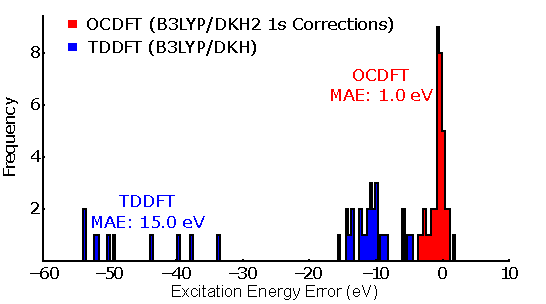
\includegraphics[scale=0.85]{ocdft_tddft_histogram.pdf}
\begin{columns}
\begin{column}{0.5\textwidth}
\begin{itemize}
\item Max Errors:
		\begin{itemize}
		\item OCDFT: $-3.7$ eV
		\item TDDFT: $-53.6$ eV
		\end{itemize}
\end{itemize}
\end{column}
\begin{column}{0.5\textwidth}
\begin{itemize}
\item MAE of Other Methods:
		\begin{itemize}
		\item EOM-CCSD: 0.9 eV
		\item SOS-CIS(D): 1.2 eV
		\end{itemize}
\end{itemize}
\end{column}
\end{columns}
\blfootnote{W. D. Derricotte and F. A. Evangelista. \textit{Phys. Chem. Chem. Phys.} \textbf{2015}}
\end{frame}

\begin{frame}{Full NEXAFS Spectral Simulation: Thymine}
\begin{itemize}
\item Transition dipole moments (TDMs) are approximated using the Kohn--Sham determinants as:
\begin{equation}
\boldsymbol{\mu}_{n0} = \bra[1]{\Phi^{(n)}} \hat{\textbf{r}}\ket[1]{\Phi^{(0)}}
\end{equation}
\item Using the approximate TDMs we can compute an oscillator strength for each transition
\begin{equation}
f_{\rm osc} = \frac{2}{3} |\mu_{n0}|^2 \omega_{n}
\end{equation}
\item Compute 10 excitations per hole for each C, N, O 1s orbital in thymine
\item Spectra plotted using Gaussians with FWHM of 0.1 eV - 0.4 eV in order to simulate natural spectroscopic broadening effects.
\end{itemize}
\blfootnote{W. D. Derricotte and F. A. Evangelista. \textit{Phys. Chem. Chem. Phys.} \textbf{2015}}
\end{frame}

\begin{frame}{Full NEXAFS Spectral Simulation: Thymine}
\begin{figure}[!t]
\centering
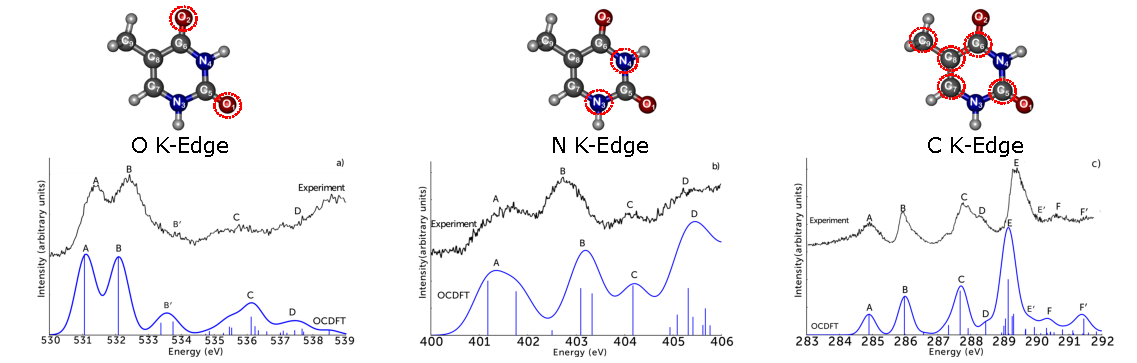
\includegraphics[scale=0.65]{thymine_all_spec.pdf}
\end{figure}
\begin{itemize}
\item \textit{Unshifted} OCDFT excitation energies provide excellent comparison to experiment
\item Average error of 0.3 eV overall compared to experimental peak maxima
\end{itemize}
\blfootnote{W. D. Derricotte and F. A. Evangelista. \textit{Phys. Chem. Chem. Phys.} \textbf{2015}}
\end{frame}

\begin{frame}{Treatment of Relativistic Effects In OCDFT}
\centering
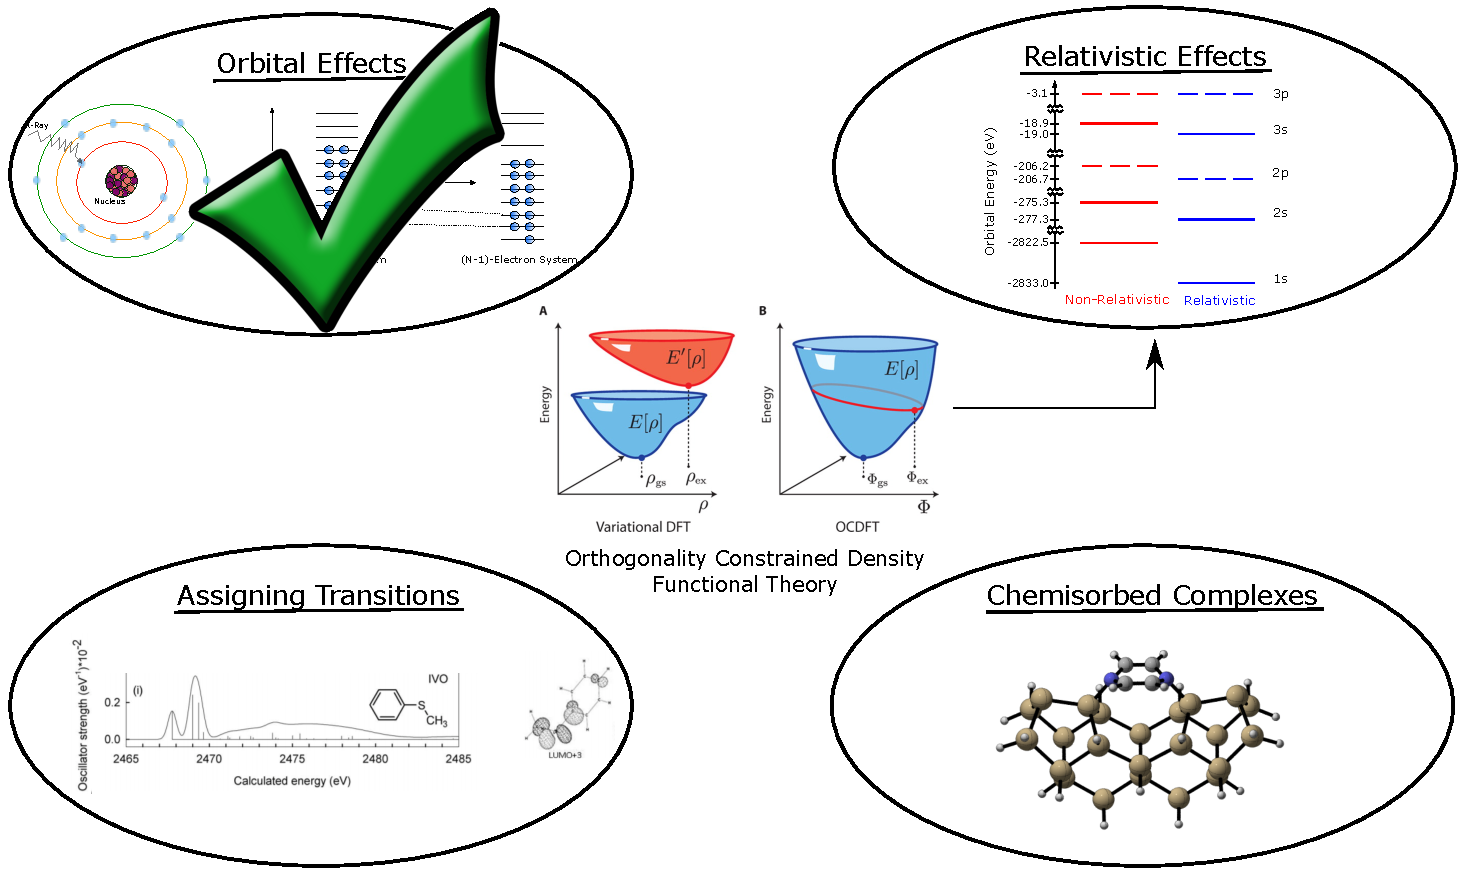
\includegraphics[width=\linewidth]{project_intro_2.pdf}
\end{frame}

\begin{frame}{Relativistic Effects in Quantum Chemistry Via 2-Component Hamiltonians}
\begin{itemize}
\item Full Dirac Relativistic equation involves a 4 component Hamiltonian ($h^{\rm D}$), 2 \textit{large} components (L), 2 \textit{small} components (S)
\begin{equation}
h^{\rm D} = 
\begin{pmatrix}
h_{LL} & h_{LS} \\
h_{SL} & h_{SS}
\end{pmatrix}
\end{equation}
\item Idea is to decouple large and small components of Dirac Hamiltonian through a Foldy-Wouthuysen (FW) unitary transformation to block diagonalize $h^{\rm D}$
\begin{equation}
U^\dagger h^{\rm D} U = 
U^\dagger
\begin{pmatrix}
h_{LL} & h_{LS} \\
h_{SL} & h_{SS}
\end{pmatrix}
 U
 =
 \begin{pmatrix}
h^{\rm FW}_{++} & 0 \\
0 & h^{\rm FW}_{--}
\end{pmatrix}
\end{equation}
\item The positive energy contribution is then isolated, which is a sum of relativistic kinetic ($T^{\rm rel}$) and potential ($V^{\rm rel}$)
\begin{equation}
h^{\rm FW}_{++} = T^{\rm rel} + V^{\rm rel}
\end{equation}
\end{itemize}
\end{frame}

\begin{frame}{Spin-Free Modified Dirac Equation}
\begin{itemize}
\item Following FW Unitary transformation, the one-electron Dirac equation can be written as:
\begin{equation}
\left(
\begin{array}{cc}
{V}                   &  {T} \\
{T} & \frac{W}{4c^2}-{T} \\ 
\end{array}
\right)
\left(
\begin{array}{c}
{C}^{\text{L}}                   \\
{C}^{\text{S}}  \\ 
\end{array}
\right)  
= \left(
\begin{array}{cc}
{S}                  &  {0}\\
{0} & \frac{{T}}{2c^2} \\ 
\end{array}
\right)
\left(
\begin{array}{c}
{C}^{\text{L}}                    \\
{C}^{\text{S}}  \\ 
\end{array}
\right)  E
\end{equation}
\item Where $W$ is the relativistic potential which is the sum of spin-free (SF) and spin-orbit (SO) contributions:
\begin{equation}
W = W^{\rm SF} + W^{\rm SO}
\end{equation}
\item Neglecting the SO term yields the \textbf{spin-free} version of the modified Dirac equation, in AO basis ($\chi_{\mu}$) $W^{SF}$ is
\begin{equation}
W^{\rm SF}_{\mu\nu} = \bra{\chi_\mu} \hat{p}\cdot (\hat{V}\hat{p}) \ket{\chi_\nu}
\end{equation}
\end{itemize}
\end{frame}

\begin{frame}{eXact-Two-Component Hamiltonian (X2C)}
\begin{itemize}
\item Given the form of the unitary tranformation of the Dirac Hamiltonian
\begin{equation}
U^\dagger h^{\rm D} U = 
 \begin{pmatrix}
h^{\rm FW}_{++} & 0 \\
0 & h^{\rm FW}_{--}
\end{pmatrix},
U = 
\begin{pmatrix}
1 & -X^{\dagger} \\
X & 1
\end{pmatrix}
\begin{pmatrix}
R & 0 \\
0 & R
\end{pmatrix}
\end{equation}
\item X and R are the \textit{coupling} and \textit{renormalization} matrices respectively and relate the MO coeffeicients of the 2c wavefunction
\begin{equation}
C^{\rm S} = XC^{\rm L} \ \ \ \ \ \ \ \ \ \ C^{\rm L} = R C^{\rm 2c}
\end{equation}
\item In X2C, these relations are used to build the relativistic kintetic and potential energy operators
\begin{align}
	T^{\text{X2C}}&= R^{\dagger} (TX +  {X}^{\dagger}T - {X}^{\dagger}TX ) R \\ 
	V^{\text{X2C}} &=  R^{\dagger}(V + \frac{1}{4c^2} X^{\dagger}W^{\text{SF}}X) R
\end{align}
\end{itemize}
\end{frame}

\begin{frame}{X2C-OCDFT}
\begin{itemize}
\item The \textit{relativistic} X2C kinetic and potential terms are now included in the OCDFT energy functional
\begin{align}
\nonumber
E^{(n)}_{\rm OCDFT}[\{\phi^{(n)}_i\}]=& \sum_{\mu \nu} D^{(n)}_{\mu \nu}(T^{\rm X2C}_{\mu \nu} + V^{\rm X2C}_{\mu \nu}) + E_{\rm coul}[\rho^{(n)}] + E^{(0)}_{\rm xc}[\rho^{(n)}]. 
\end{align}
\item X2C one-electron operator is formed before the SCF cycle and added to the \textit{nonrelativistic} two-electron operators
\end{itemize}
\blfootnote{P. Verma; W. D. Derricotte; and F. A. Evangelista. \textit{J. Chem. Theory Comput.} \textbf{2016}}
\end{frame}

\begin{frame}{X2C-OCDFT Benchmark}
\begin{columns}
\begin{column}{0.5\textwidth}
\begin{figure}
\centering
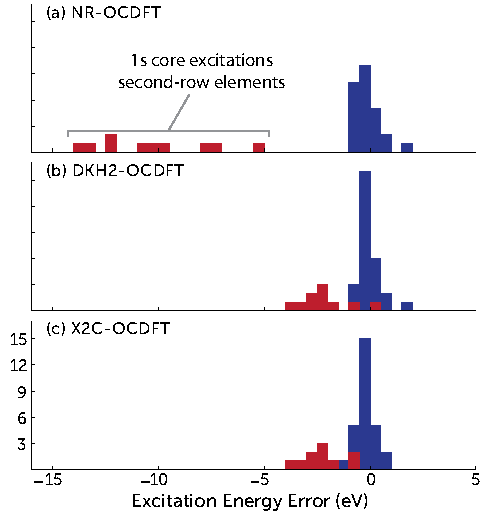
\includegraphics[width=\linewidth]{figure_3.pdf}
\end{figure}
\end{column}
\begin{column}{0.5\textwidth}
\begin{itemize}
\item Benchmarked using 37 core-excitations from 13 different molecules
\item Calculations done using B3LYP functional and fully uncontracted aug-cc-pVDZ basis set
\item MAE for X2C-OCDFT:
		\begin{itemize}
		\item 1$^{\text{st}}$ row: 0.3 eV
		\item 2$^{\text{nd}}$ row: 0.7eV
		\end{itemize}
\end{itemize}
\end{column}
\end{columns}
\blfootnote{P. Verma; W. D. Derricotte; and F. A. Evangelista. \textit{J. Chem. Theory Comput.} \textbf{2016}}
\end{frame}

\begin{frame}{Relativistic Effects vs. Correlation Effects}
\begin{table}[t!]
\begin{tabular}{ccc}
\toprule
Transitions & Relativistic (eV) & Correlation (eV) \\
\midrule
First row 1s & 0.2 & 0.6 \\
Second row 1s & 8.0 & 3.4 \\
Second row 2p & 0.5 & 1.1 \\
All & 2.2 & 1.3 \\
\bottomrule
\end{tabular}
\label{table:CorrRel}
\end{table}
\begin{align}
\text{Rel} &= \text{OCDFT}^{\text{NR}}(E^{\text{B3LYP}}_{\text{xc}}) - \text{OCDFT}^{\text{X2C}}(E^{\text{B3LYP}}_{\rm xc}) \\
\text{Corr} &= \text{OCDFT}^{\text{X2C}}(E^{\text{B3LYP}}_{\text{xc}}) - \text{OCDFT}^{\text{X2C}}(E^{\text{HF}}_{\text{x}})
\end{align}
\begin{itemize}
\item Proper treatment of electron correlation is more important for 1$^{\text{st}}$ row elements
\item Quickly outpaced by relativistic effects for 2$^{\text{nd}}$ row
\item Proper treatment of relativistic effects will be extremely important for transition metals
\end{itemize}
\blfootnote{P. Verma; W. D. Derricotte; and F. A. Evangelista. \textit{J. Chem. Theory Comput.} \textbf{2016}}
\end{frame}

\begin{frame}{K-Edge of Tetracoordinated Ti Complexes}
\begin{figure}
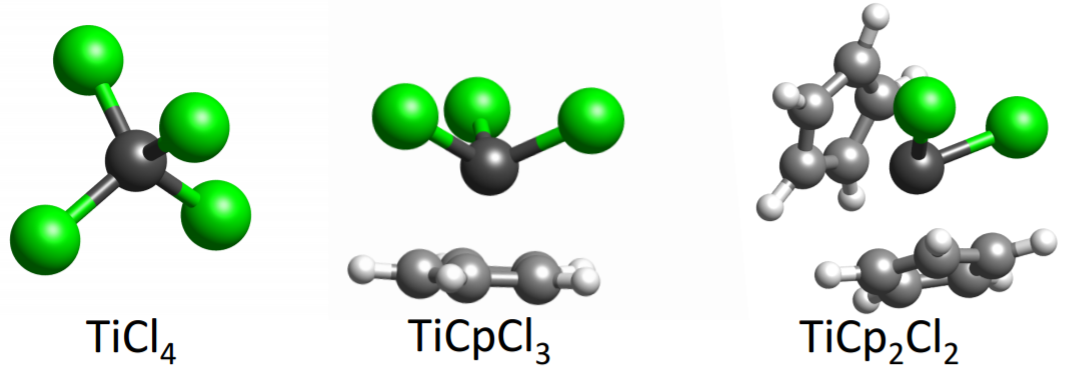
\includegraphics[scale=0.3]{Ti_structs.png}
\end{figure}

\begin{table}[!t]
\footnotesize
\begin{tabular}{cccccc}
\toprule
State & \multicolumn{2}{c}{TDDFT} & \multicolumn{2}{c}{OCDFT} & Exp. \\ \cmidrule(r){2-3}  \cmidrule(l){4-5}
 & NR & DKH2 & NR & X2C  \\
\midrule
1 & $-$107.9& $-$78.6& $-$35.6& $-$5.0 & \multirow{5}{*}{$\left. \vphantom{\begin{tabular}{c}3\\3\\3 \\3\end{tabular}}\right\}$ 4969.2} \\
2 & $-$107.9& $-$78.6& $-$35.5& $-$4.5 \\
3 & $-$107.0& $-$77.6& $-$36.4& $-$5.7 \\
4 & $-$106.9& $-$77.6& $-$35.3& $-$4.8 \\
5 & $-$107.0& $-$77.7& $-$36.3& $-$5.7 \\
\bottomrule
	\label{table:Ti-complex}
\end{tabular}
\end{table}
\begin{itemize}
\item Pre-edge feature is calculated within $\approx$ 5.0 eV of experiment
\end{itemize}
\blfootnote{P. Verma; W. D. Derricotte; and F. A. Evangelista. \textit{J. Chem. Theory Comput.} \textbf{2016}}
\end{frame}

\begin{frame}{Pre-edge Features of Tetracoordinated Ti Complexes}
\begin{figure}
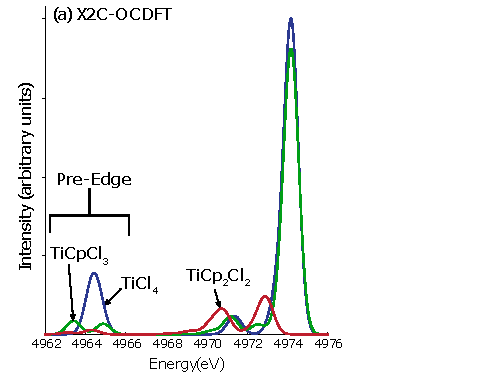
\includegraphics[scale=1.0]{ti_pre_edge_1.pdf}
\end{figure}
\begin{itemize}
\item Pre-edge intensity drop after adding Cp rings to coordination
\end{itemize}
\blfootnote{P. Verma; W. D. Derricotte; and F. A. Evangelista. \textit{J. Chem. Theory Comput.} \textbf{2016}}
\end{frame}

\begin{frame}{Pre-edge Features of Tetracoordinated Ti Complexes}
\begin{figure}
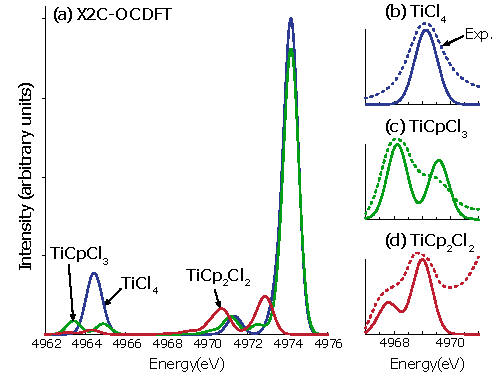
\includegraphics[scale=1.0]{ti_pre_edge_2.pdf}
\end{figure}
\begin{itemize}
\item Peak splitting of pre-edge after adding Cp rings to coordination
\end{itemize}
\blfootnote{P. Verma; W. D. Derricotte; and F. A. Evangelista. \textit{J. Chem. Theory Comput.} \textbf{2016}}
\end{frame}

\begin{frame}{Particle Orbital Analysis of Pre-Edge TiCl$_4$}
 \begin{figure}
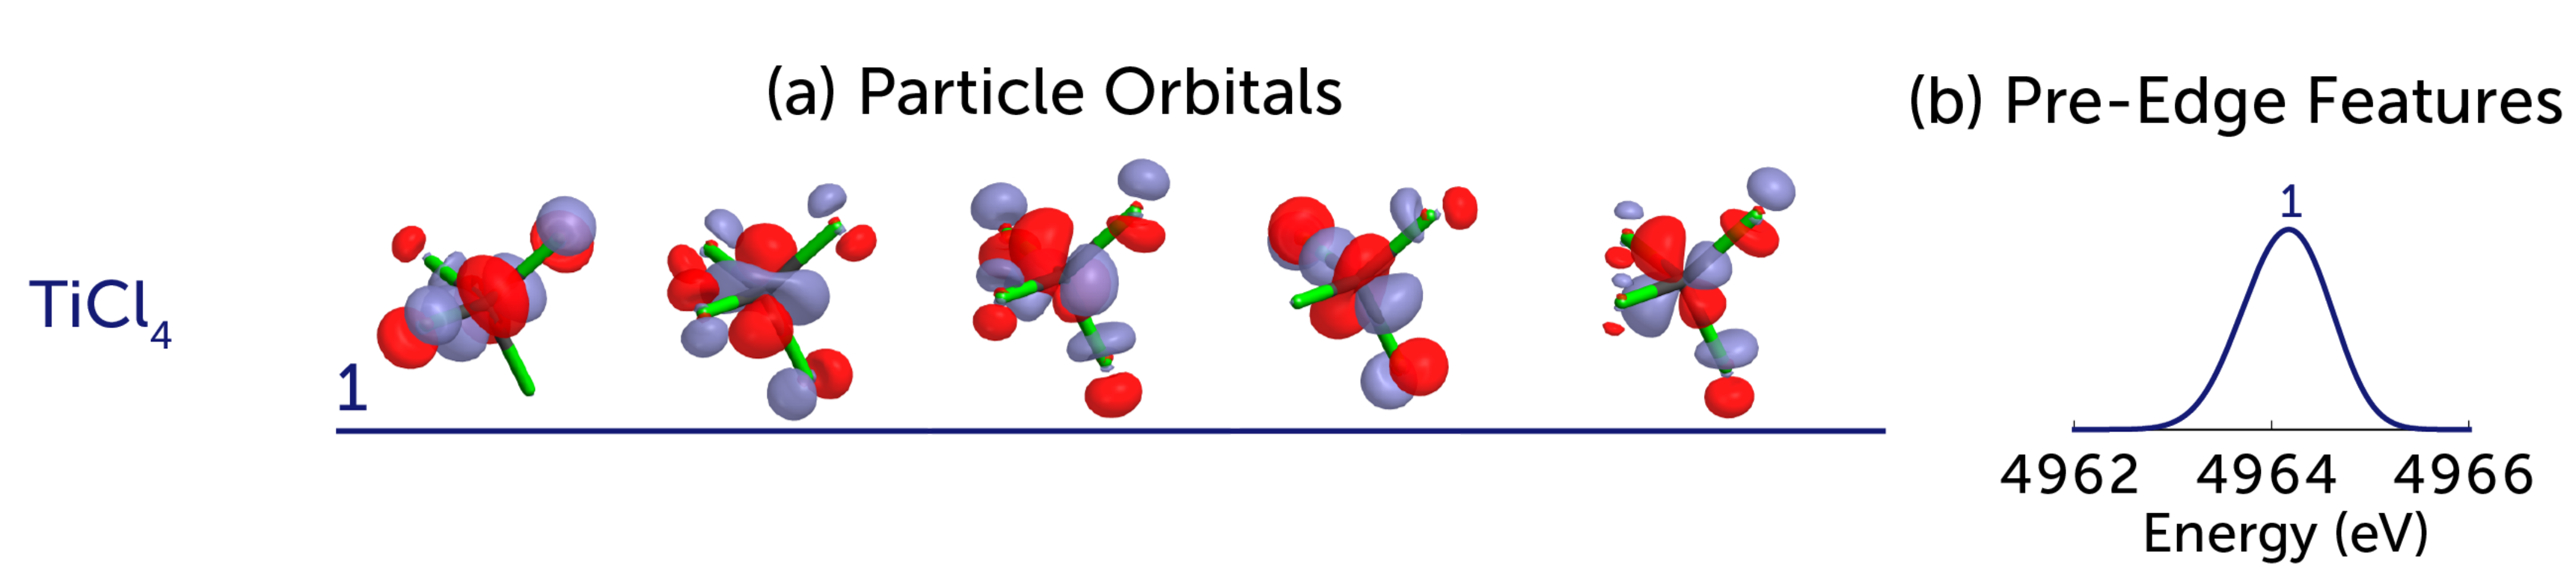
\includegraphics[scale=0.15]{ticl4_preedge.png}
\end{figure}
\begin{table}
\footnotesize
\begin{tabular}{c@{\hskip 1in}c@{\hskip 1in}c}
\toprule
State &   \multicolumn{2}{c}{\textbf{TiCl$_4$}}   \\
& Energy & $f$ \\
\cmidrule(r){2-3}
1 & 4964.2 & 0.0945\\
2 & 4964.7 & 0.0940\\
3 & 4963.5 & 0.0002\\
4 & 4964.4 & 0.0947\\
5 & 4963.5 & 0.0000\\
\bottomrule
\end{tabular}
\end{table}
\begin{itemize}
\item All particle orbitals have similar character (i.e. Ti d and Cl p)
\end{itemize}
\blfootnote{P. Verma; W. D. Derricotte; and F. A. Evangelista. \textit{J. Chem. Theory Comput.} \textbf{2016}}
\end{frame}

\begin{frame}{Particle Orbital Analysis of Pre-Edge TiCpCl$_3$}
 \begin{figure}
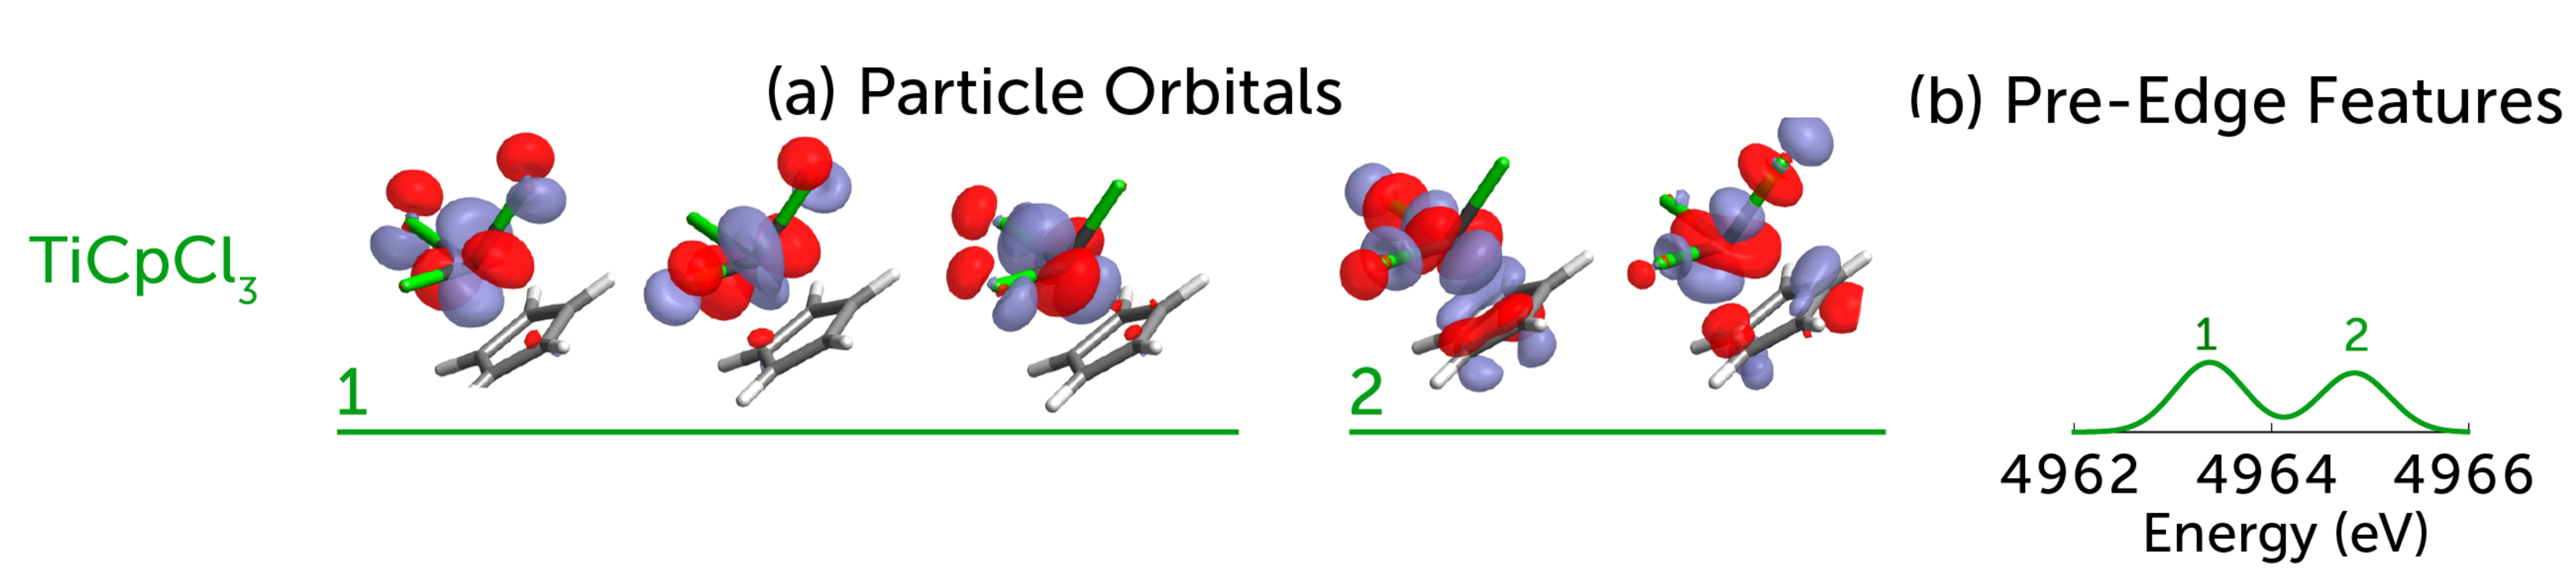
\includegraphics[scale=0.15]{ticpcl3_preedge.png}
\end{figure}
\begin{table}
\footnotesize
\begin{tabular}{c@{\hskip 1in}c@{\hskip 1in}c}
\toprule
State &   \multicolumn{2}{c}{\textbf{TiCpCl$_3$}}   \\
& Energy & $f$ \\
\cmidrule(r){2-3}
1 & 4963.4 & 0.0202\\
2 & 4963.4 & 0.0191\\
3 & 4963.5 & 0.0164\\
4 & 4964.9 & 0.0220\\
5 & 4963.9 & 0.0217\\
\bottomrule
\end{tabular}
\end{table}
\begin{itemize}
\item States with significant Cp ring contributions are pushed to higher energy
\end{itemize}
\blfootnote{P. Verma; W. D. Derricotte; and F. A. Evangelista. \textit{J. Chem. Theory Comput.} \textbf{2016}}
\end{frame}

\begin{frame}{Particle Orbital Analysis of Pre-Edge TiCp$_2$Cl$_2$}
 \begin{figure}
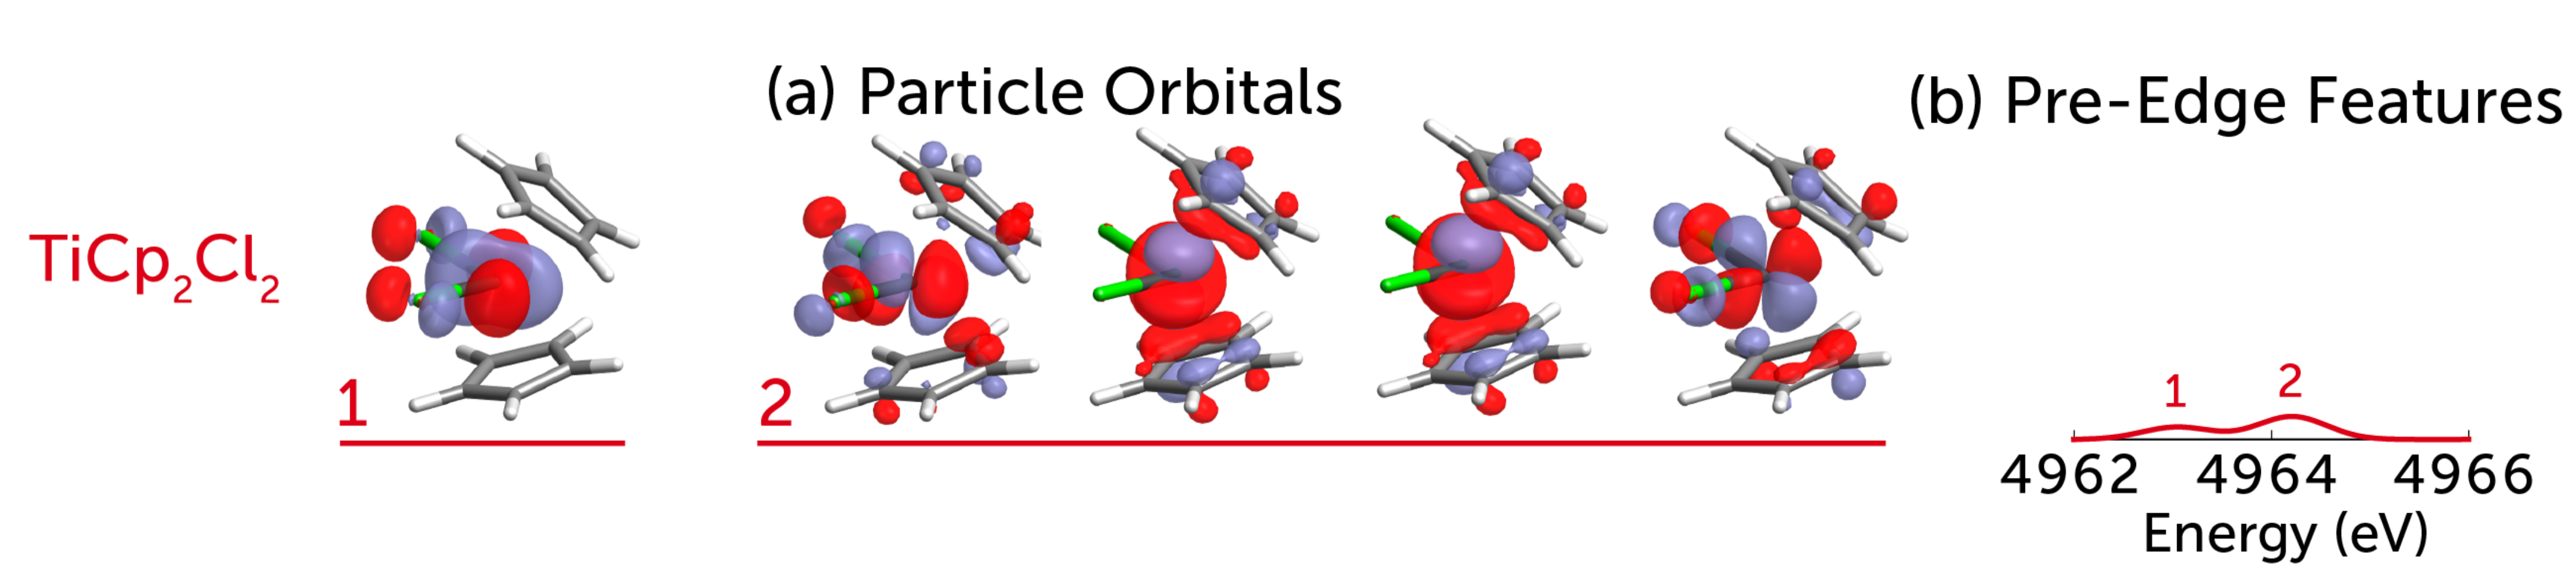
\includegraphics[scale=0.15]{ticp2cl2_preedge.png}
\end{figure}
\begin{table}
\footnotesize
\begin{tabular}{c@{\hskip 1in}c@{\hskip 1in}c}
\toprule
State &   \multicolumn{2}{c}{\textbf{TiCp$_2$Cl$_2$}}   \\
& Energy & $f$ \\
\cmidrule(r){2-3}
1 & 4963.1 & 0.0078\\
2 & 4964.3 & 0.0121\\
3 & 4964.4 & 0.0009\\
4 & 4964.4 & 0.0000\\
5 & 4964.3 & 0.0055\\
\bottomrule
\end{tabular}
\end{table}
\begin{itemize}
\item States with significant Cp ring contributions are pushed to higher energy
\end{itemize}
\blfootnote{P. Verma; W. D. Derricotte; and F. A. Evangelista. \textit{J. Chem. Theory Comput.} \textbf{2016}}
\end{frame}

\begin{frame}{Further Investigation of Pre-Edge Intensity}
\begin{itemize}
\item Pre-edge intensity will be evaluated using the following methods:
		\begin{itemize}
		\item Natural population analysis using JANPA software
		\item Atomic decomposition of the total dipole moment
		\end{itemize}
\item We can decompose the total dipole moment in the following fashion
\begin{equation}
\boldsymbol\mu_{0n} = \bra[1]{\Phi^{(n)}}\hat{\mathbf{r}} \ket[1]{\Phi^{(0)}} = \sum_{\mu\nu} D^{0n}_{\mu\nu} \bra{\chi_\mu} \hat{\mathbf{r}} \ket{\chi_\nu}
\end{equation}
\item From here we can do a restricted sum over donor/acceptor atom and angular momentum shell
\begin{equation}
\boldsymbol\mu_{0n} (\mathrm{A}_{l_\mathrm{A}} \rightarrow \mathrm{B}_{l_\mathrm{B}}) = \sum_{\mu \in \mathrm{A}_{l_\mathrm{A}}}\sum_{\nu \in \mathrm{B}_{l_\mathrm{B}}} D^{0n}_{\mu\nu} \bra{\chi_\mu} \mathbf{r} \ket{\chi_\nu}
\end{equation}
\end{itemize}
\blfootnote{P. Verma; W. D. Derricotte; and F. A. Evangelista. \textit{J. Chem. Theory Comput.} \textbf{2016}}
\end{frame}

\begin{frame}{Further Investigation of Pre-Edge Intensity}
\begin{table}
\footnotesize
	\caption*{Natural Population Analysis}
	\resizebox{0.8\linewidth}{!}{
	\begin{tabular}{lrrrrrrrrr}
		\toprule
		 &  \multicolumn{3}{c}{$\Delta$Ti$_\text{p}$}  & \multicolumn{3}{c}{$\Delta$Cl$_\text{p}$} &  \multicolumn{3}{c}{$\Delta$Ti$_\text{d}$}  \\ \cmidrule(lr){2-4} \cmidrule(lr){5-7} \cmidrule(lr){8-10}
		State & {\text{TiCl$_4$}}  & {\text{TiCpCl$_3$}} & {\text{TiCp$_2$Cl$_2$}}& {\text{TiCl$_4$}}  & {\text{TiCpCl$_3$}} & {\text{TiCp$_2$Cl$_2$}}& {\text{TiCl$_4$}}  & {\text{TiCpCl$_3$}} & {\text{TiCp$_2$Cl$_2$}} \\ \cmidrule(lr){2-4} \cmidrule(lr){5-7} \cmidrule(lr){8-10}
1	&	0.0107	&	0.0066	&	0.0097	&	-0.2184	&	-0.0597	&	0.0051	&	1.1348	&	1.1614	&	1.2586	\\
\bottomrule
\end{tabular}}
\end{table}

\begin{table}
	\centering
	\caption*{Atomic Decomposition of Dipole Moments}
	\resizebox{0.6\linewidth}{!}{
	\begin{tabular}{lcccc}
		\toprule
		Contribution                  &     $\mu_x$ &     $\mu_y$ &     $\mu_z$ & $|\boldsymbol\mu|$ \\ \midrule
\multicolumn{5}{c}{{\bf{State 1}}}   \\
Ti$_{\rm s}$ $\rightarrow$ Ti$_{\rm p}$ & $-$0.000395 & $-$0.000079 & $-$0.000113 & 0.000418 \\
Cl$_{\rm p}$ $\rightarrow$ Cl$_{\rm p}$ & +0.000062 & +0.000012 & +0.000018 & 0.000066 \\
Ti$_{\rm s}$ $\rightarrow$ Cl$_{\rm p}$ & $-$0.000006 & +0.000003 & $-$0.000064 & 0.000064 \\
Other       & $-$0.000007 & +0.000002 & +0.000073 & 0.000073 \\
\bottomrule
\end{tabular}}
\end{table}
\begin{itemize}
\item Population analysis shows that the transitions are 1s$\rightarrow$ 3d
\item Largest dipole contribution is Ti$_{\text{s}}$ $\rightarrow$ Ti$_{\text{d}}$
\end{itemize}
\blfootnote{P. Verma; W. D. Derricotte; and F. A. Evangelista. \textit{J. Chem. Theory Comput.} \textbf{2016}}
\end{frame}

\begin{frame}{Overview of Dissertation Work}
\centering
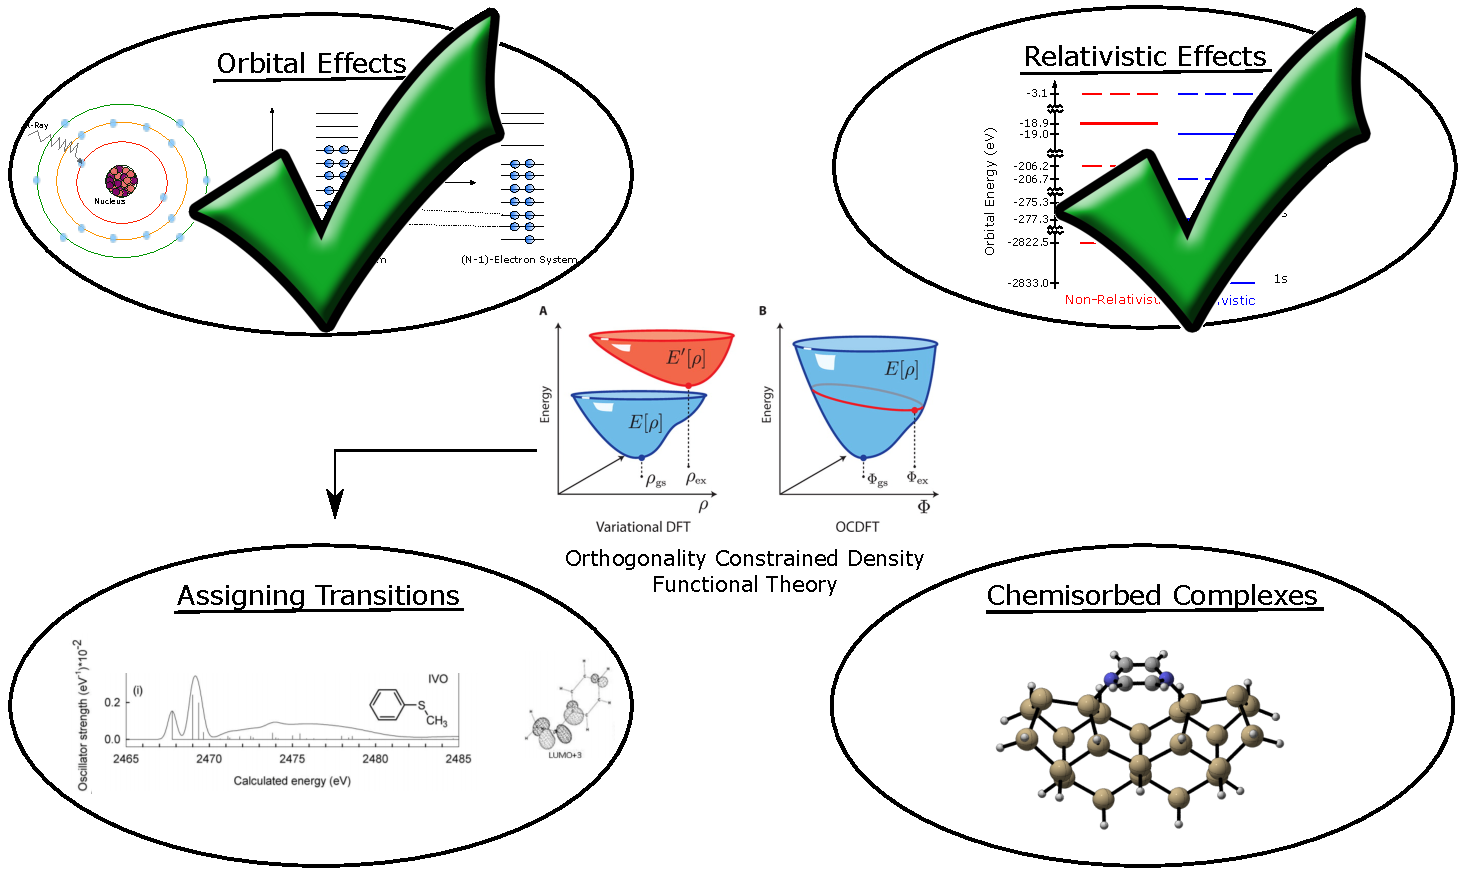
\includegraphics[width=\linewidth]{project_intro_3.pdf}
\end{frame}

\begin{frame}{Assigning the Character of Particle Orbitals}
\centering
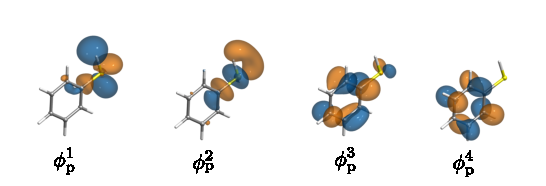
\includegraphics[width=\linewidth]{assigning_particles.pdf}
\begin{itemize}
\item $\phi^1_{\rm p}$ and $\phi^2_{\rm p}$ clearly have contributions from both $\sigma^*_{\rm S-C}$ and 
$\sigma^*_{\rm S-H}$ how do you make a definitive assignment?
\item How to differentiate between the two unique $\pi^*_{\rm C=C}$ orbitals?
\item Desirable to find method to quantify localized orbital contributions
\end{itemize}
\end{frame}

\begin{frame}{Localized Intrinsic Valence Virtual Orbitals}
\centering
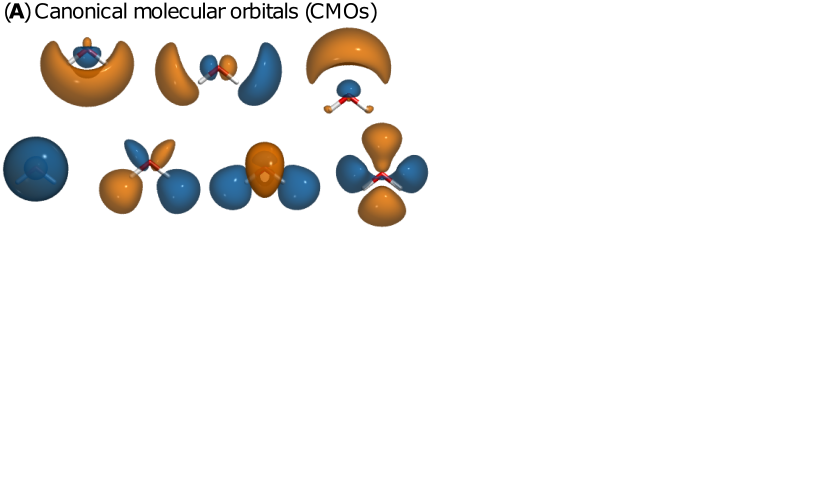
\includegraphics[width=0.75\linewidth]{livvo_procedure_1.png}
\begin{itemize}
\item Start with a set of virtual canonical molecular orbitals (CMOs) expanded in an atom-centered basis $\{\chi_{\mu}\}$
\begin{equation}
|\phi_a\rangle = \sum_{\mu}^{N_\mathrm{AO}} |\chi_{\mu} \rangle C_{\mu a}, \quad a = 1,\ldots,N_\mathrm{vir}
\end{equation}
\end{itemize}
\end{frame}

\begin{frame}{Localized Intrinsic Valence Virtual Orbitals}
\centering
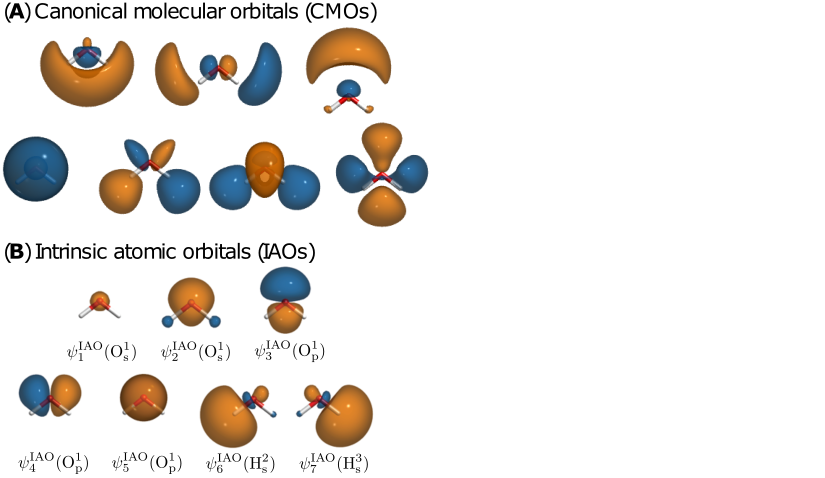
\includegraphics[width=0.75\linewidth]{livvo_procedure_2.png}
\begin{itemize}
\item Evaluate overlap ($\mathbf{S}$) with set of Intrinsic Atomic Orbitals (IAOs) 
\end{itemize}
\begin{equation}
(\mathbf{S})_{a\rho} = \langle \phi_a | \psi_{\rho}^\mathrm{IAO} \rangle
\end{equation}
\end{frame}

\begin{frame}{Localized Intrinsic Valence Virtual Orbitals}
\centering
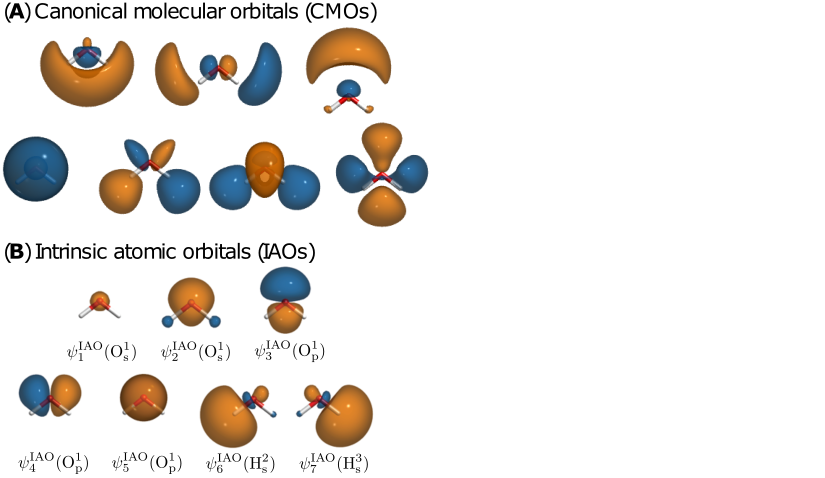
\includegraphics[width=0.75\linewidth]{livvo_procedure_2.png}
\begin{itemize}
\item Perform SVD of overlap matrix to get orthogonal tranformation matrices $\mathbf{U}$ and $\mathbf{V}$
\end{itemize}
\begin{equation}
\mathbf{S} = \mathbf{U} \boldsymbol{
\sigma} \mathbf{V}^{\dagger}
\end{equation}
\end{frame}


\begin{frame}{Localized Intrinsic Valence Virtual Orbitals}
\centering
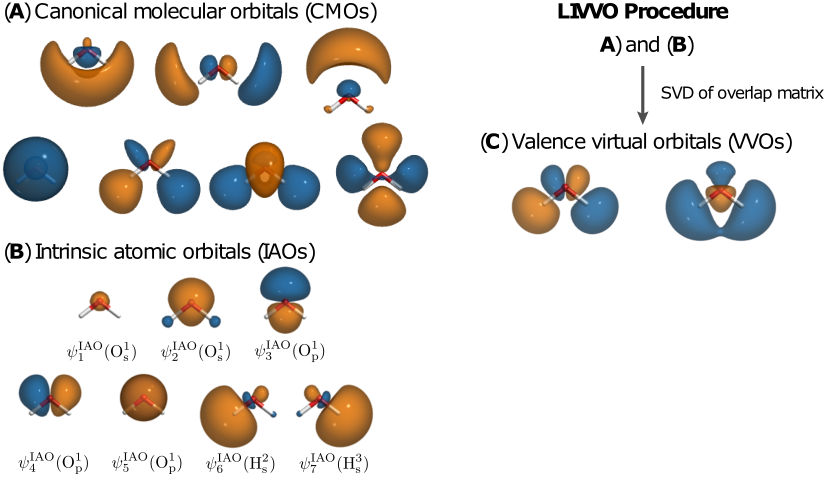
\includegraphics[width=0.75\linewidth]{livvo_procedure_3.png}
\begin{itemize}
\item Use $\mathbf{U}$ to transform canonical virtuals into valence virtual orbitals (VVOs):
\end{itemize}
\begin{equation}
| \psi^{\rm VVO}_v \rangle = \sum_a^{N_\mathrm{vir}} | \phi_a \rangle U_{av}, \quad v = 1, \ldots, N_{\rm VVO}.
\end{equation}
\end{frame}

\begin{frame}{Localized Intrinsic Valence Virtual Orbitals}
\centering
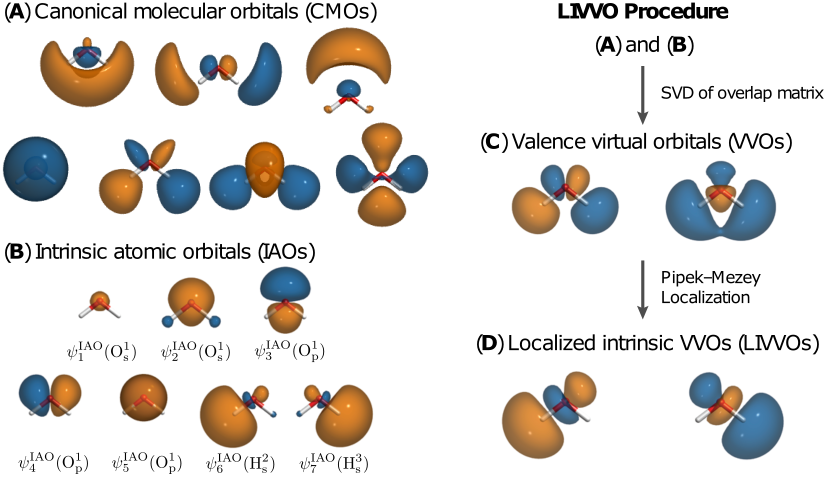
\includegraphics[width=0.75\linewidth]{livvo_procedure_4.png}
\begin{itemize}
\item Pipek-Mezey localization can be employed in order to yield an orbital set that represents each valence antibonding interaction in the molecular environment
\end{itemize}
\end{frame}

\begin{frame}{Determining Atomic Character of IAOs}
\begin{itemize}
\item Atomic character is assigned using a Mulliken Population Analysis
\begin{columns}
\begin{column}{0.5\linewidth}
\begin{figure}
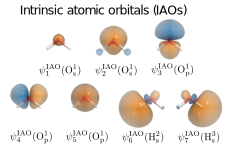
\includegraphics[scale=0.6]{water_IAOs.png}
\end{figure}
\end{column}
\begin{column}{0.5\linewidth}
\vspace{-2mm}
\begin{table}[b]
\renewcommand{\arraystretch}{1.2}
\footnotesize
\centering
%\caption{Atom-centered gross orbital populations [GP$_{A_l}(\rho)$] for the seven IAOs of water. Calculations were performed at the B3LYP/jun-cc-pVTZ level of theory.}
\caption*{Gross Populations}
\resizebox{0.8\linewidth}{!}{
\begin{tabular}{r@{\hskip6pt}r@{\hskip6pt}r@{\hskip6pt}r@{\hskip6pt}r@{\hskip6pt}r@{\hskip6pt}r@{\hskip6pt}r}
\toprule
$A_{l}$ & $\psi^{\rm IAO}_1$ & $\psi^{\rm IAO}_2$ & $\psi^{\rm IAO}_3$ & $\psi^{\rm IAO}_4$& $\psi^{\rm IAO}_5$& $\psi^{\rm IAO}_6$& $\psi^{\rm IAO}_7$ \\[3pt]
\midrule
O$_\mathrm{s}^1$ & 1.00 & 1.16 & 0.00 & 0.00 & 0.00 & $-$0.08 & $-$0.08 \\
O$_\mathrm{p}^1$ & 0.00 & 0.00 & 1.04 & 1.11 & 1.00 & $-$0.07 & $-$0.07 \\
H$^2_\mathrm{s}$ &0.00 & $-$0.08 & $-$0.02 & $-$0.05 & 0.00 & 1.18&  $-$0.03\\
H$^3_\mathrm{s}$ & 0.00 & $-$0.08 & $-$0.02 & $-$0.05 & 0.00 & $-$0.03 & 1.18\\
\bottomrule
\end{tabular}}
\label{tab:iao_atomic}
\end{table}
\end{column}
\end{columns}
\item We compute the population matrix ($P_{\mu\nu}$) as:
\begin{equation}
P_{\mu\nu}(\rho) = \tilde{C}_{\mu \rho} S_{\mu\nu} \tilde{C}_{\nu \rho}, \quad \rho = 1, \ldots, N_\mathrm{IAO}
\end{equation}
\item Gross populations on each atom $A$ and angular momentum shell $l$ are obtained via partial sums of $P_{\mu\nu}$
\begin{equation}
\mathrm{GP}_{A_{l}}(\rho)  = \sum_{\mu \in A_{l}} \sum_{\nu}^{N_\mathrm{AO}} P_{\mu\nu}(\rho) 
\end{equation}
\item character of each IAO chosen as maximum $\mathrm{GP}_{A_{l}}(\rho)$ contribution
\end{itemize}
\end{frame}

\begin{frame}{Using IAOs to Classify LIVVOs}
\begin{itemize}
\item Overlap of each LIVVO ($\psi_l^{\rm LIVVO}$) with the IAOs ($\psi^{\rm IAO}_{\rho}$) is evaluated:
\begin{equation}
S'_{l \rho} = | \langle \psi_l^{\rm LIVVO} | \psi^{\rm IAO}_{\rho} \rangle |^2
\end{equation}
\item Assign orbital character ($\sigma$,$\pi$,\ldots) of LIVVOs based on atomic character (s,p,\ldots) of IAOs
\begin{equation*}
\begin{split}
\vcenter{\hbox{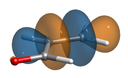
\includegraphics[width = 2.5cm]{img_1a}}} =& 
\, 0.20 \, \psi^{\rm IAO}(\rm C^2_s) + 0.24 \, \psi^{\rm IAO}(\rm C^2_p) \\
& + 0.20 \, \psi^{\rm IAO}(\rm C^3_s)  + 0.25 \, \psi^{\rm IAO}(\rm C^3_p) = \sigma^*_{\rm C^2-C^3}\\
\\
\vcenter{\hbox{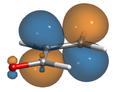
\includegraphics[width = 2.25cm]{img_1b}}} =& \,
 0.47 \, \psi^{\rm IAO}(\rm C^2_p)  + 0.51 \,  \psi^{\rm IAO}(\rm C^3_p)  = \pi^*_{\rm C^2-C^3}
\end{split}
\end{equation*}
\end{itemize}
\end{frame}

\begin{frame}{Assigning Orbital Character of OCDFT Particle Orbitals}
\begin{itemize}
\item Character of the particle orbital $\phi_{\rm p}^{(n)}$ by evaluating its overlap with each LIVVO ($\psi^{\rm LIVVO}_l$)
\begin{equation}
\label{eq:part_livvo_overlap}
\Omega_{\mathrm{p}l}^{(n)} = | \langle \phi^{(n)}_\mathrm{p} | \psi^{\rm LIVVO}_l \rangle |^2.
\end{equation}
\begin{figure}
\vspace{-5mm}
\centering
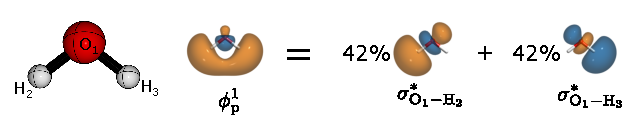
\includegraphics[width=0.9\textwidth]{water_example.pdf}
\end{figure}
\item Total valence character can be quantified by summing all LIVVO contributions. (84\% for above H$_2$O example)
\begin{equation}
t^{\mathrm{val},(n)}_\mathrm{p} = \sum_{l}^{N_\mathrm{LIVVO}} \Omega_{\mathrm{p}l}^{(n)}.
\end{equation}
\end{itemize}
\end{frame}

\begin{frame}{Assigning Transitions in S K-edge of Ethanethiol and Benzenethiol}
\begin{itemize}
\item Spectra are calculated with OCDFT at the B3LYP/jun-cc-pVTZ level of theory
\end{itemize}
\begin{figure}
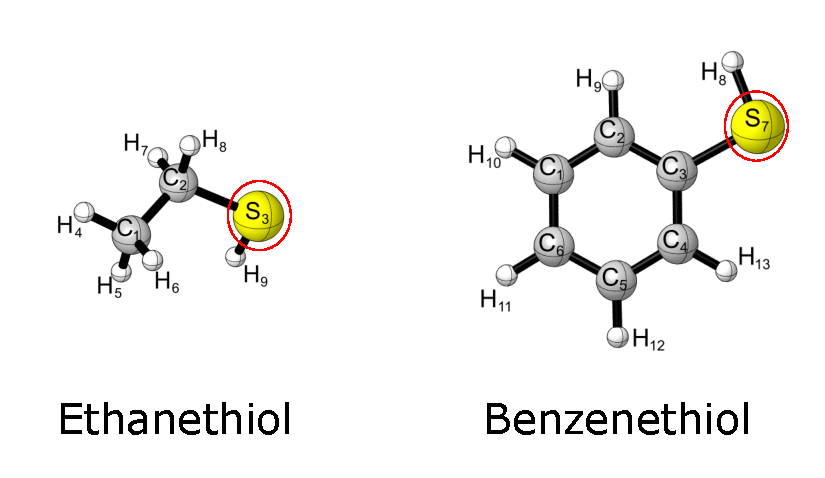
\includegraphics[width=0.8\textwidth]{ethane_benzenethiol_header.pdf}
\end{figure}
\end{frame}

\begin{frame}{What are the local contributions to $\phi^1_{\rm p}$ and $\phi^2_{\rm p}$?}
\begin{figure}
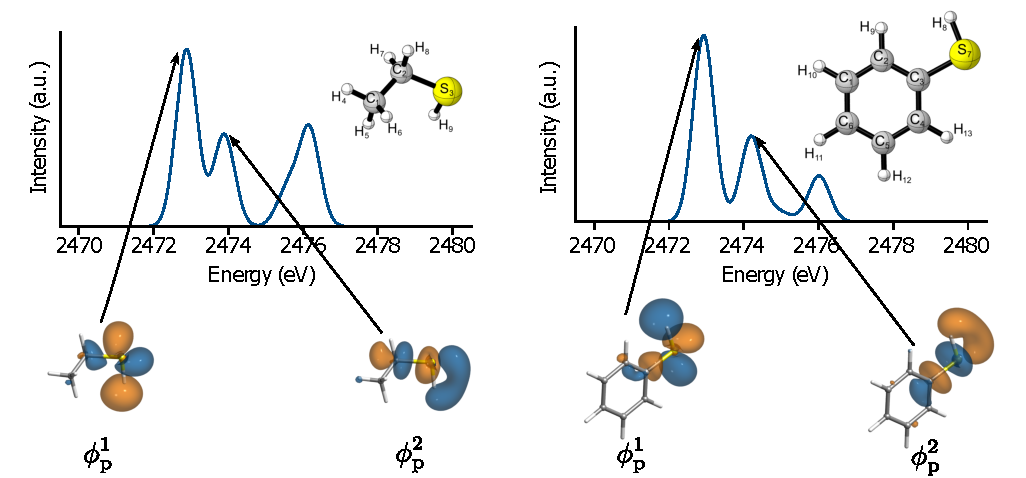
\includegraphics[width=\textwidth]{ethane_benzenethiol_spectra.pdf}
\end{figure}
\begin{itemize}
\item Particle orbitals contain orbital character along ${\rm S-C}$ and ${\rm S-H}$
\item What is the contribution of the thiol bond to each excited state?
\end{itemize}
\end{frame}

\begin{frame}{What are the local contributions to $\phi^1_{\rm p}$ and $\phi^2_{\rm p}$?}
\begin{figure}
\centering
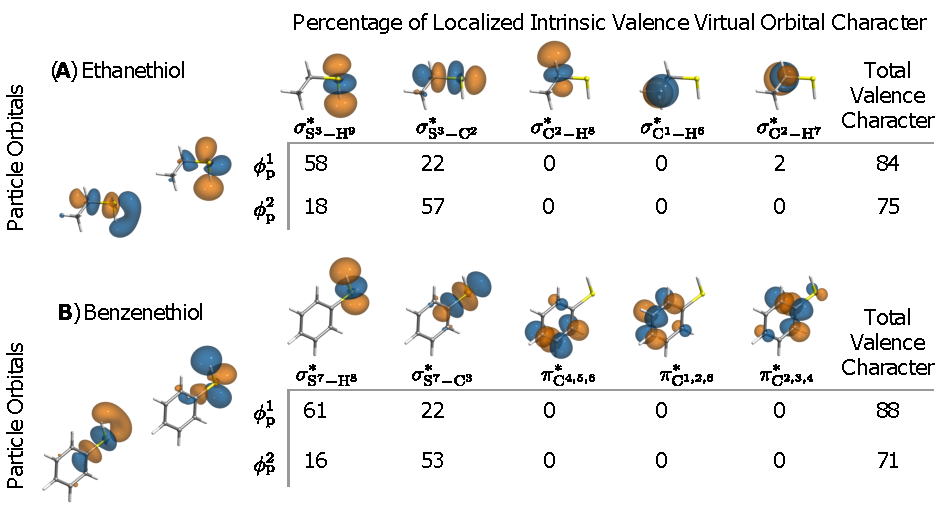
\includegraphics[width=0.8\textwidth]{alt_ethane_benzenethiol_livvo.pdf}
\end{figure}
\begin{itemize}
\item LIVVO analysis yields \textit{unambiguous} assignment for each particle orbital
\item Thiol bond is large contributor to first peak, weak contributor to second peak
\end{itemize}
\end{frame}

\begin{frame}{Other Contributions to the S K-Edge}
\begin{figure}
\centering
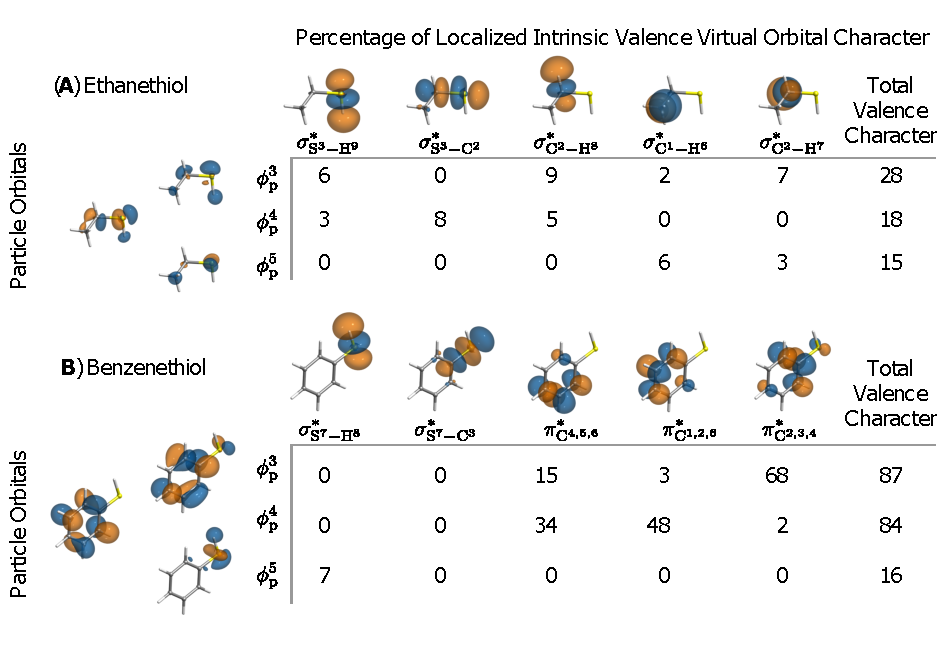
\includegraphics[width=0.8\textwidth]{other_livvo_contributions.pdf}
\end{figure}
\begin{itemize}
\item $\phi^3_{\rm p}$ and $\phi^4_{\rm p}$ localized away from S atom in benzenethiol, results in lower intensity
\end{itemize}
\end{frame}

\begin{frame}{Effect of Hydrogen Bonding on O K-Edge of Water}
\begin{itemize}
\item Spectra are calculated with OCDFT at the B3LYP/jun-cc-pVTZ level of theory
\end{itemize}
\begin{figure}
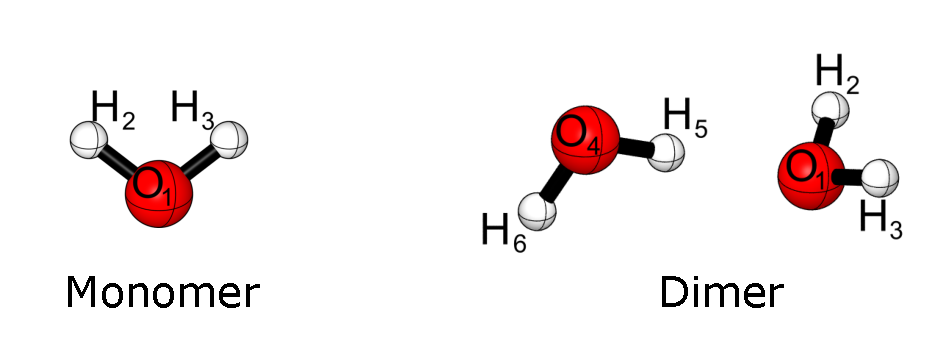
\includegraphics[width=0.8\textwidth]{water_monomer_dimer_header.pdf}
\end{figure}
\end{frame}

\begin{frame}{Effect of Hydrogen Bonding on O K-Edge of Water}
\begin{figure}
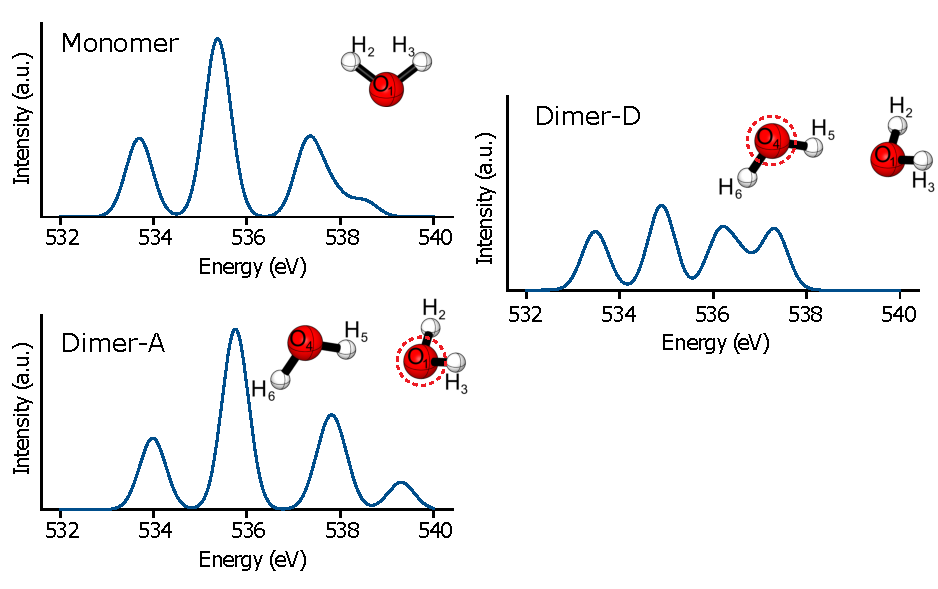
\includegraphics[width=0.8\textwidth]{water_spectra_slide.pdf}
\end{figure}
\begin{itemize}
\item Accepting H-bond (Dimer-A) has small effect on spectral features, donating H-bond (Dimer-D) has significant effect
\end{itemize}
\end{frame}

\begin{frame}{Effect of Hydrogen Bonding on O K-Edge of Water}
\begin{figure}
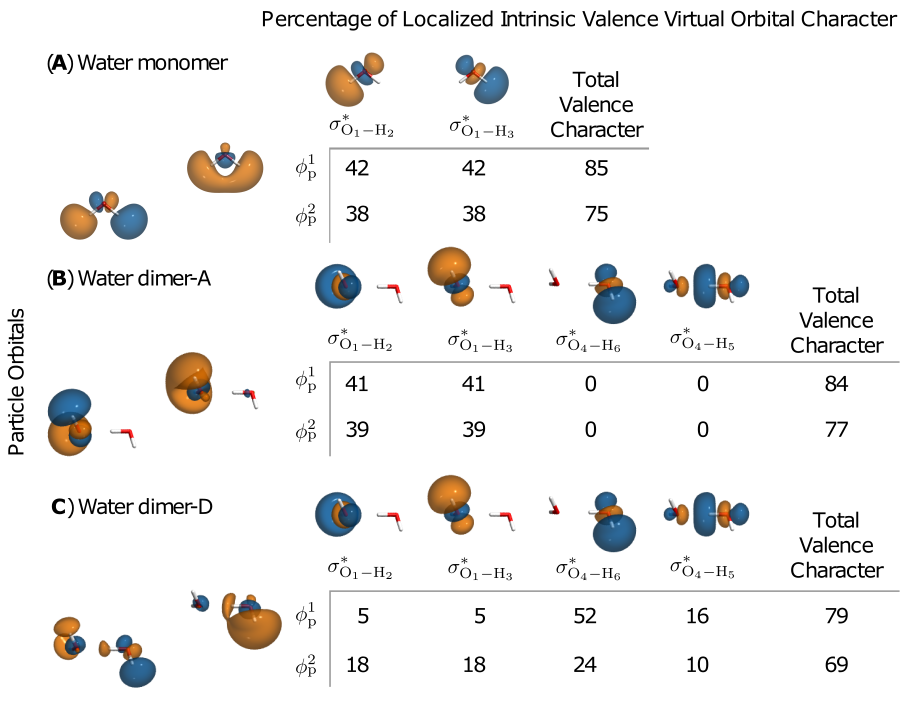
\includegraphics[width=0.8\textwidth]{water_livvo_slide.png}
\end{figure}
\end{frame}

\begin{frame}{Overview of Dissertation Work}
\centering
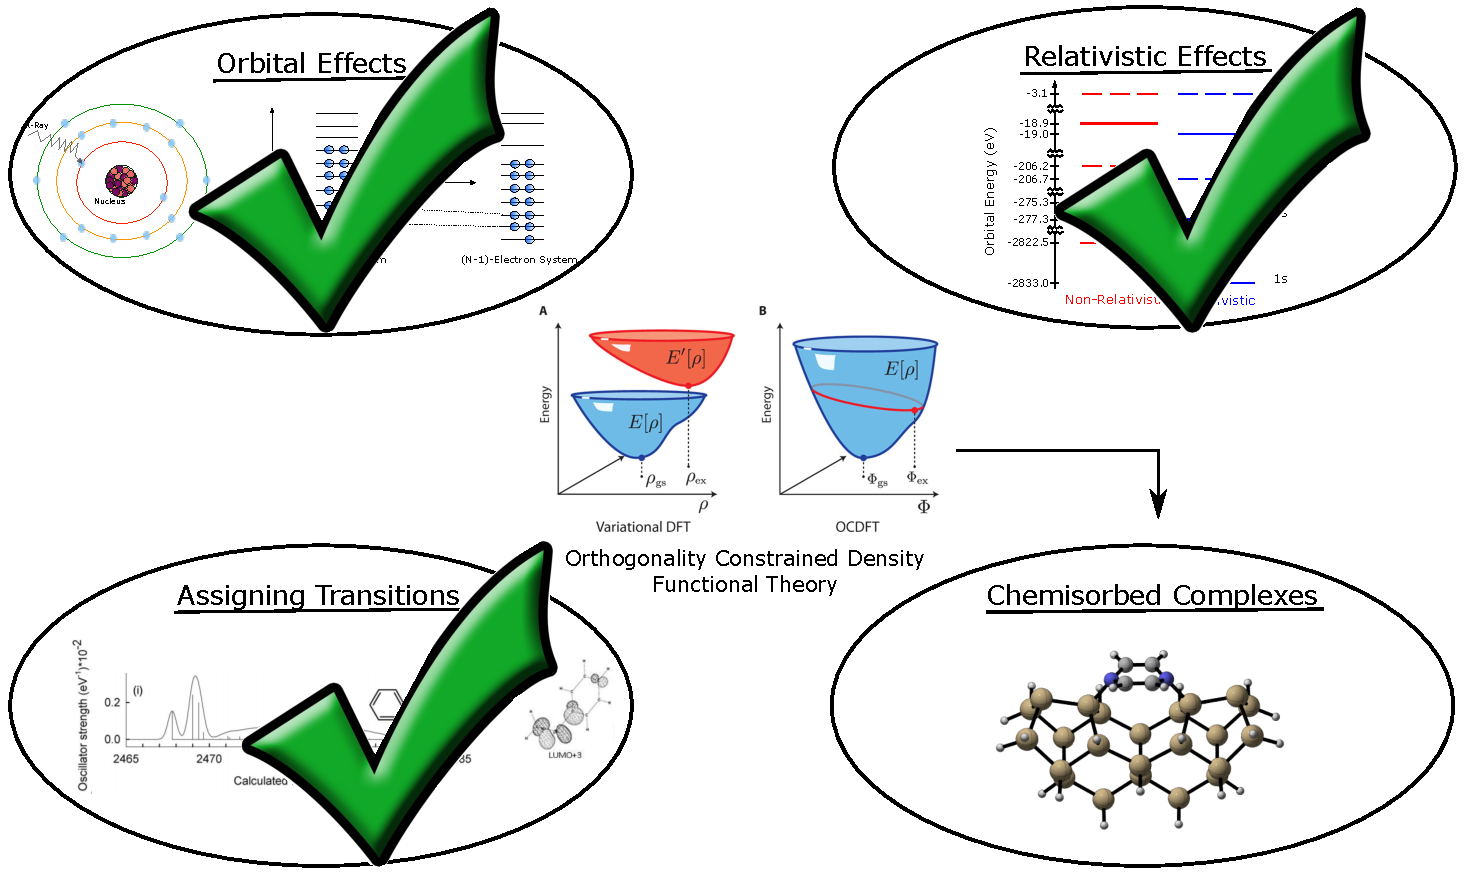
\includegraphics[width=\linewidth]{project_intro_4.pdf}
\end{frame}

\begin{frame}{Organic Core-Excitations in Chemisorbed Molecules}
\begin{figure}
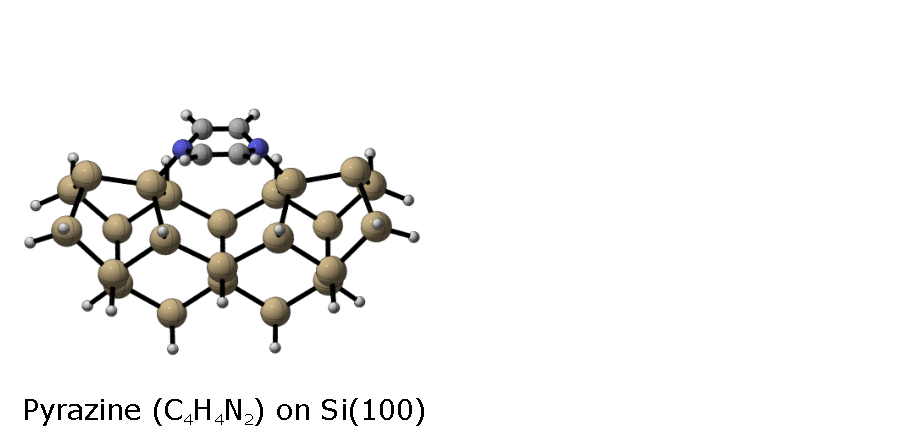
\includegraphics[width=0.8\textwidth]{pyrazine_si_100_slide_1.pdf}
\end{figure}
\begin{itemize}
\item Appropriate surface cluster models contain at least 10 or more surface atoms
\end{itemize}
\end{frame}

\begin{frame}{Organic Core-Excitations in Chemisorbed Molecules}
\begin{figure}
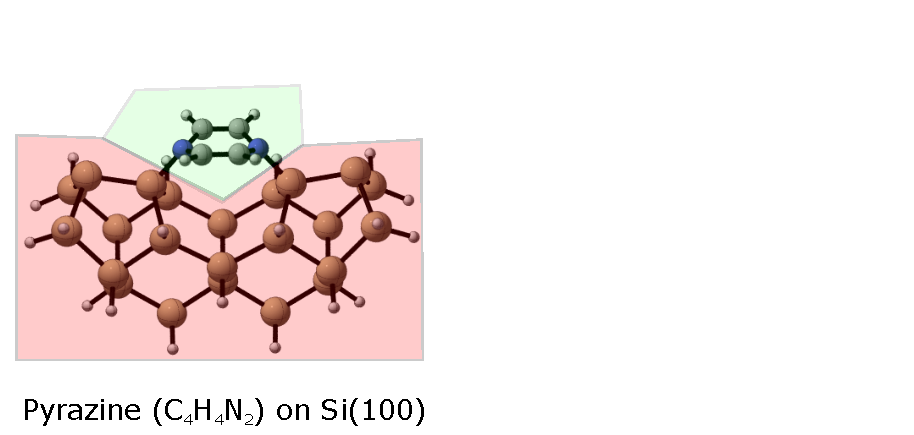
\includegraphics[width=0.8\textwidth]{pyrazine_si_100_slide_2.pdf}
\end{figure}
\begin{itemize}
\item Appropriate surface cluster models contain at least 10 or more surface atoms
\item Model complexes contain the organic \textcolor{green}{adsorbate} attached to a \textcolor{red}{surface cluster}
\end{itemize}
\end{frame}

\begin{frame}{Organic Core-Excitations in Chemisorbed Molecules}
\begin{figure}
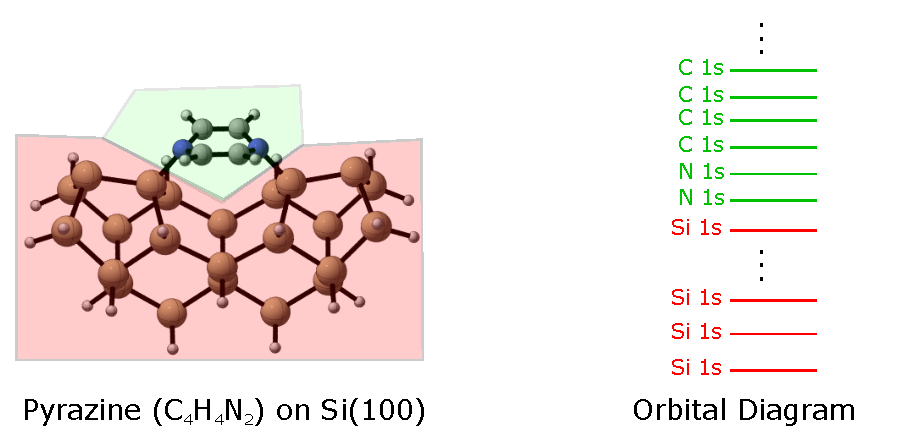
\includegraphics[width=0.8\textwidth]{pyrazine_si_100_slide_3.pdf}
\end{figure}
\begin{itemize}
\item Lowest energy core orbitals are associated with the \textcolor{red}{surface cluster}
\item Presents an algorithmic challenge for original OCDFT algorithm
\item Need a method to specifically target core orbitals of the \textcolor{green}{organic adsorbate}
\end{itemize}
\end{frame}

\begin{frame}{Maximum Subspace Occupation (MSO) Approach}
\begin{itemize}
\item Consider a set of atomic orbital basis functions ($\varphi_{s}$) ordered by atom center, principal quantum number, and angular momentum
\item We can build an operator that spans a subset ($s$) of AOs
\begin{equation}
\hat{\Gamma}_{s} = \sum_{s}\ket[1]{\varphi_{s}}\bra[1]{\varphi_{s}}
\end{equation}
\item Evaluate an atomic orbital occupation number ($\Omega_i$) for each occupied molecular orbital ($\phi_i$) within the desired subspace
\begin{equation}
\Omega_i = \bra[1]{\phi_i} \hat{\Gamma}_{s} \ket[1]{\phi_i} = \sum_{s} \braket[1]{\phi_i}{\varphi_{s}}\braket[1]{\varphi_{s}}{\phi_i}.
\end{equation}
\item Hole orbital ($\phi_h$) is now chosen from a subset of the occupied orbitals where $\Omega_i$ is greater than a user-defined occupation threshold parameter
\end{itemize}
\end{frame}

\begin{frame}{MSO-OCDFT: CO Example}
\centering
\includegraphics{CO_projection.pdf}
\begin{itemize}
\item C 1s orbital is targeted based on its occupation in the C 1s atomic orbital subset
\item Note: Due to locality of core orbitals, threshold can be set fairly high
\end{itemize}
\end{frame}


\begin{frame}{MSO-OCDFT: Consistency of Energy and $f_{\rm osc}$}
\begin{itemize}
\item Test calculations done on CCl$_4$ using both the standard algorithm and MSO-OCDFT
\begin{table}
\centering
\caption*{First 3 C core excitations in CCl$_4$}
\resizebox{0.7\linewidth}{!}{
\begin{tabular}{ccccc}
\hline
\hline
State & \multicolumn{2}{c}{OCDFT}& \multicolumn{2}{c}{MSO-OCDFT}  \\
\hline 
& $\omega$ (eV) & f$_{\rm osc}$ & $\omega$ (eV) & f$_{\rm osc}$ \\
\hline 
1 & 292.0002 & 0.0000 & 292.0005 & 0.0000\\
2 & 292.7093 & 0.0384 & 292.7097 & 0.0384 \\
3 & 292.6669 & 0.0385 & 292.6659 & 0.0385\\
\hline
\hline
\end{tabular}}
\label{tab:CCl4}
\end{table}
\item Negligible differences between the two results
\item Validates that this is a good approximation to full orthogonal set of solutions
\end{itemize}
\end{frame}

\begin{frame}{C and N K-Edge of Pyrazine}
\centering
\includegraphics[width=\linewidth]{pyrazine_chemisorbed_c_kedge.pdf}
\begin{itemize}
\item Able to target C and N core efficiently with MSO-OCDFT
\item 10 excited states were targeted for each spectrum
\item Without MSO:
		\begin{itemize}
		\item 230 Si Excitations would have been necessary to calculate before N K-edge
		\item 230 Si + 20 N excitations would have been necessary before the C K-edge
		\end{itemize}
\end{itemize}
\end{frame}

\begin{frame}{Concluding Remarks}
\begin{itemize}
\item OCDFT has been extended and proven successful for calculating core-excited
\item Full Treatment of relativistic effects were included via the X2C Hamiltonian and 
\item A Localized set of orbitals has been introduced and use to quantify local contributions to the OCDFT particle orbitals
\item An approach to target specific hole orbitals based on occupation in an AO subset has been introduced and allows for the calculation core-excited states of chemisorbed organic complexes.
\end{itemize}
\end{frame}

\begin{frame}{Professional Acknowledgments}
\includegraphics[width=\linewidth]{pro_acknow.pdf}
\begin{itemize}
\item ALL CURRENT EVANGELISTA GROUP MEMBERS! (Pictured above)
\item Former Evangelista Lab Group Members
		\begin{itemize}
		\item Dr. Prakash Verma
		\item Kevin Hannon
		\end{itemize}
\item Funding from the NSF Graduate Research Fellowship Program
\item Initial Funding from the NIH Initiative to Maximize Student Development (IMSD)
\end{itemize}
\end{frame}

\begin{frame}{Family Acknowledgments}
\includegraphics[width=\linewidth]{fam_acknow.pdf} \\ \\
``Family and friendships are two of the greatest facilitators of happiness.'' -- John C. Maxwell
\end{frame}

\begin{frame}{Thank You!}
\centering
\includegraphics[width=\linewidth]{project_intro__done.pdf}
\end{frame}

\end{document}